

\subsection{Jet kinematics}

The following sections summarize jet kinematics for inclusive jets and dijets at 2.76 TeV, for inclusive jets at 5.02 TeV, and for dijets in each asymmetry class at 2.76 TeV.

\subsubsection{Jet kinematics at 2.76 TeV}
\label{app:kinematics_run1}

The kinematic observables of jets in pp and PbPb 2.76 TeV events (solid markers) are compared with Monte Carlo (hatched marks). All spectra have been normalized to unity. Comparing the jet spectra observed in PbPb data (pp data) and in {\sc pythia+hydjet} ({\sc pythia}) samples, a reasonable agreement in the overall shape is found.
 
 
 \begin{figure}[h!]
 \begin{center}
 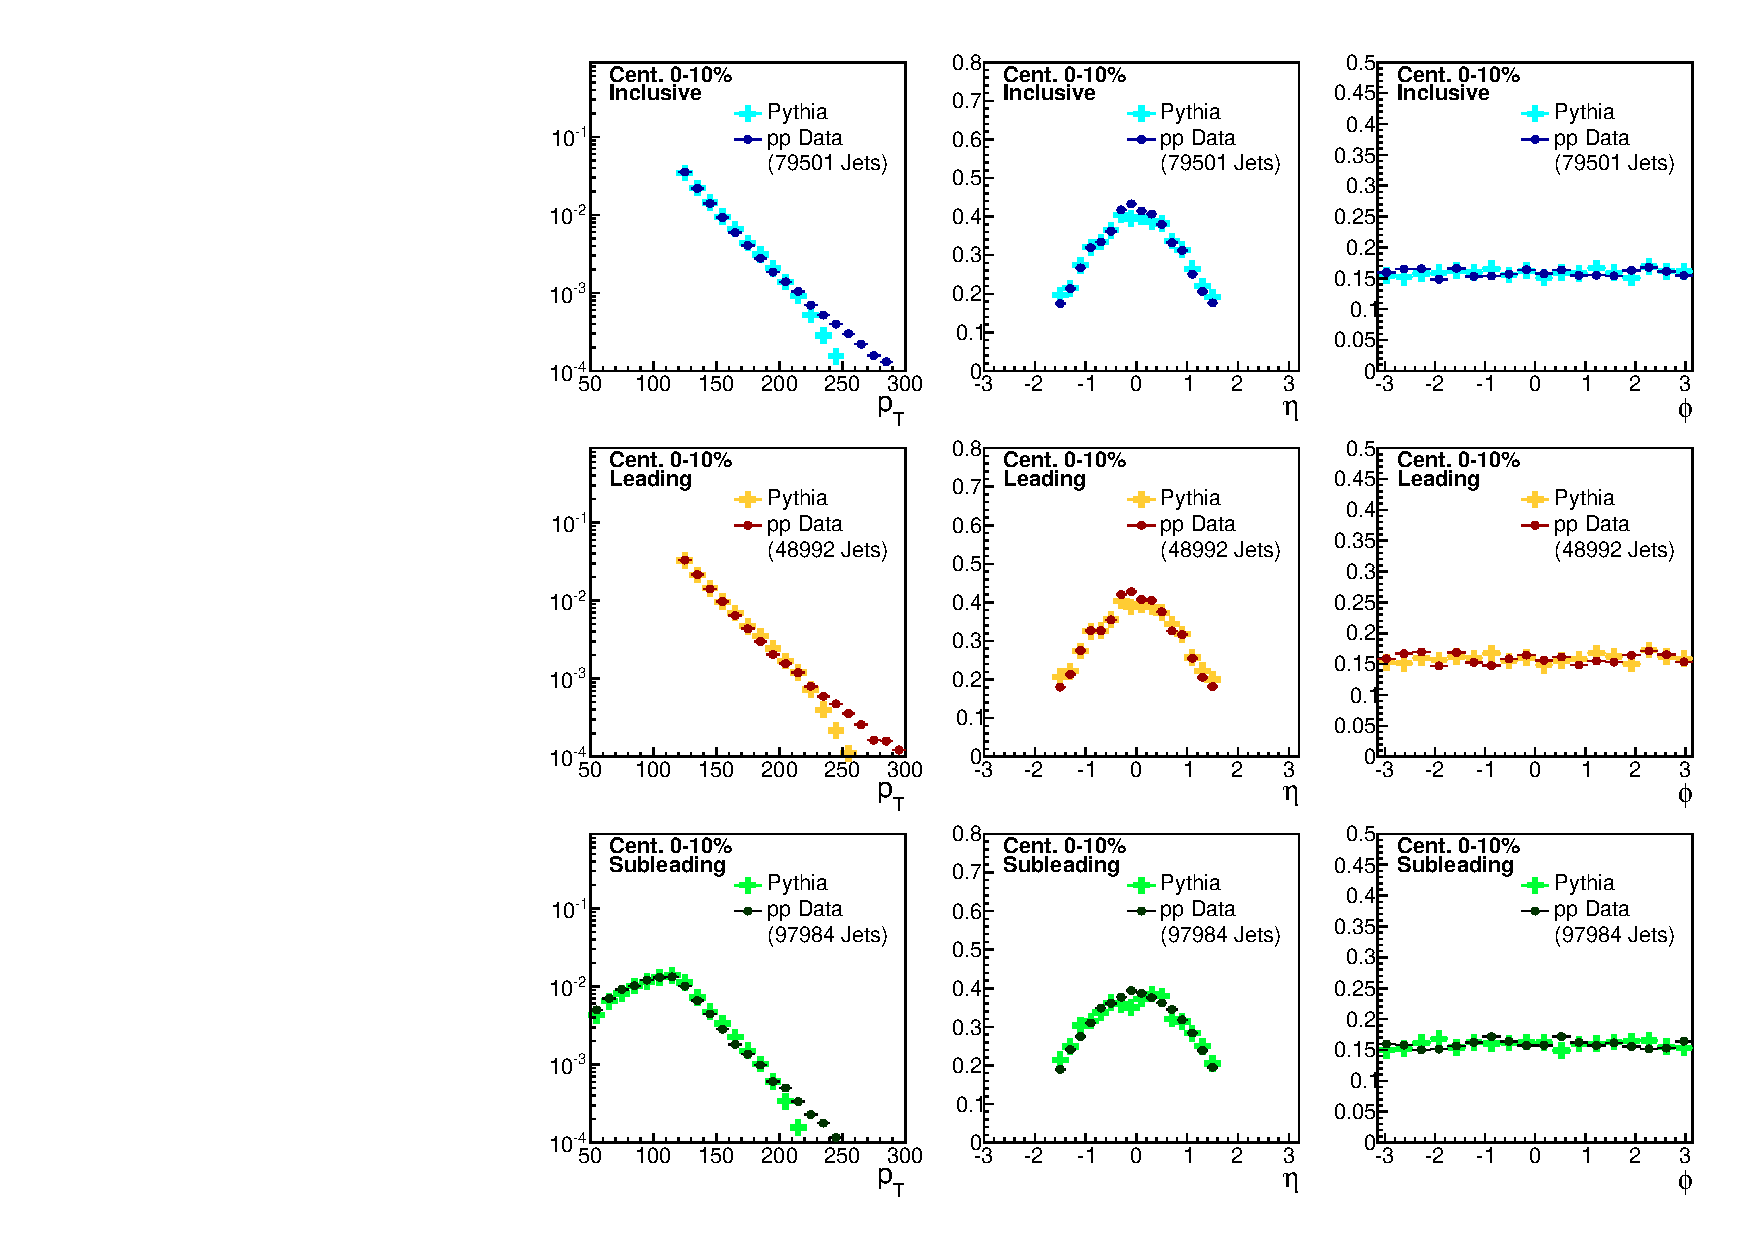
\includegraphics[width=.75\textwidth]{figures/Appendices/JetSpectra_MC_Data_Pythia_RecoJet_JetEtaCut16.pdf}
 \caption{Distribution of transverse momentum, pseudorapidity, and azimuthal distribution of all jet selections for Pythia data compared to {\sc pythia} simulation.}
  \label{fig:ppJetPt}
 \end{center}
 \end{figure}
 

 
  \begin{figure}[h!]
 \begin{center}
 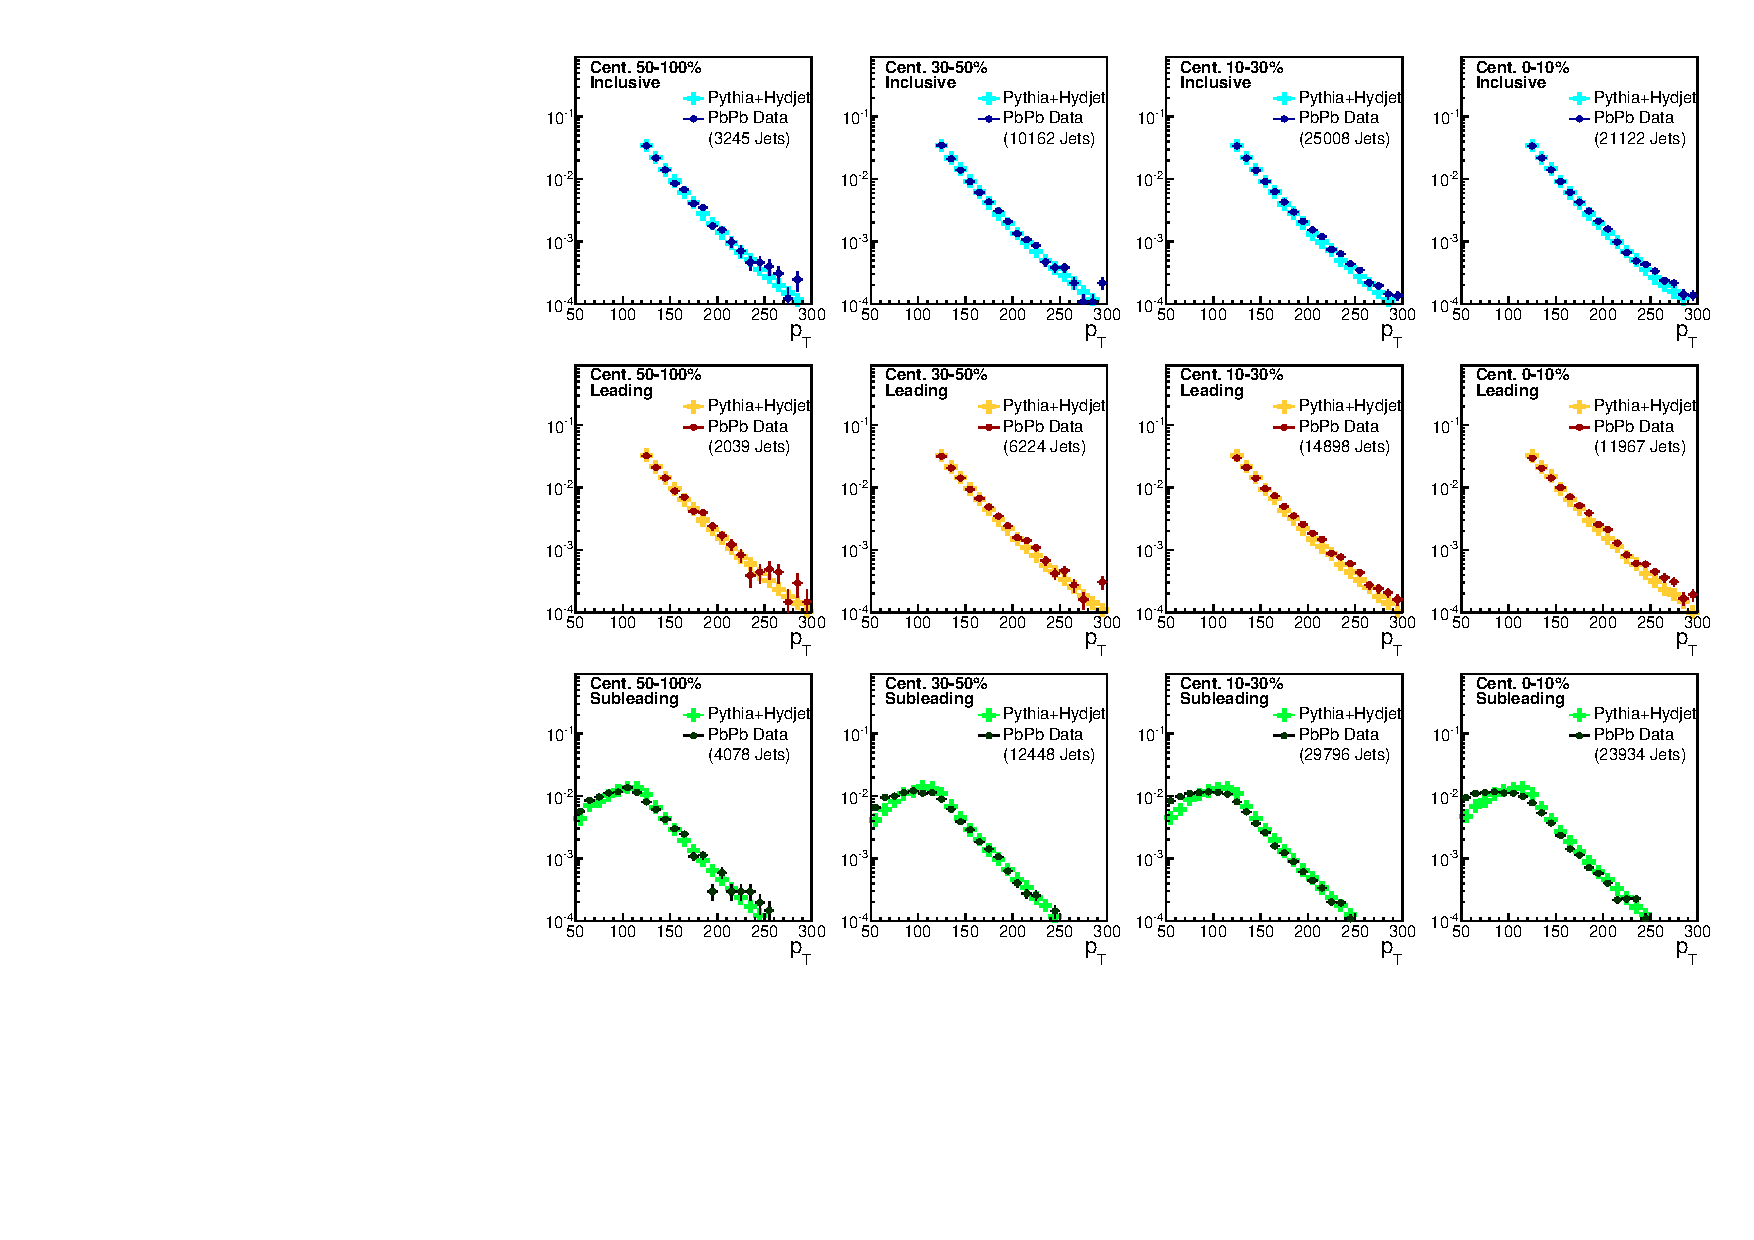
\includegraphics[width=1\textwidth]{figures/Appendices/JetSpectra_MC_Data_HydJet_RecoJet_JetEtaCut16.pdf}
 \caption{Transverse momentum distribution of all jet selections for PbPb data  at 2.76 TeV compared to {\sc pythia+hydjet} simulation.}
 \label{fig:PbPbJetPt}
 \end{center}
 \end{figure}


 \begin{figure}[h!]
 \begin{center}
 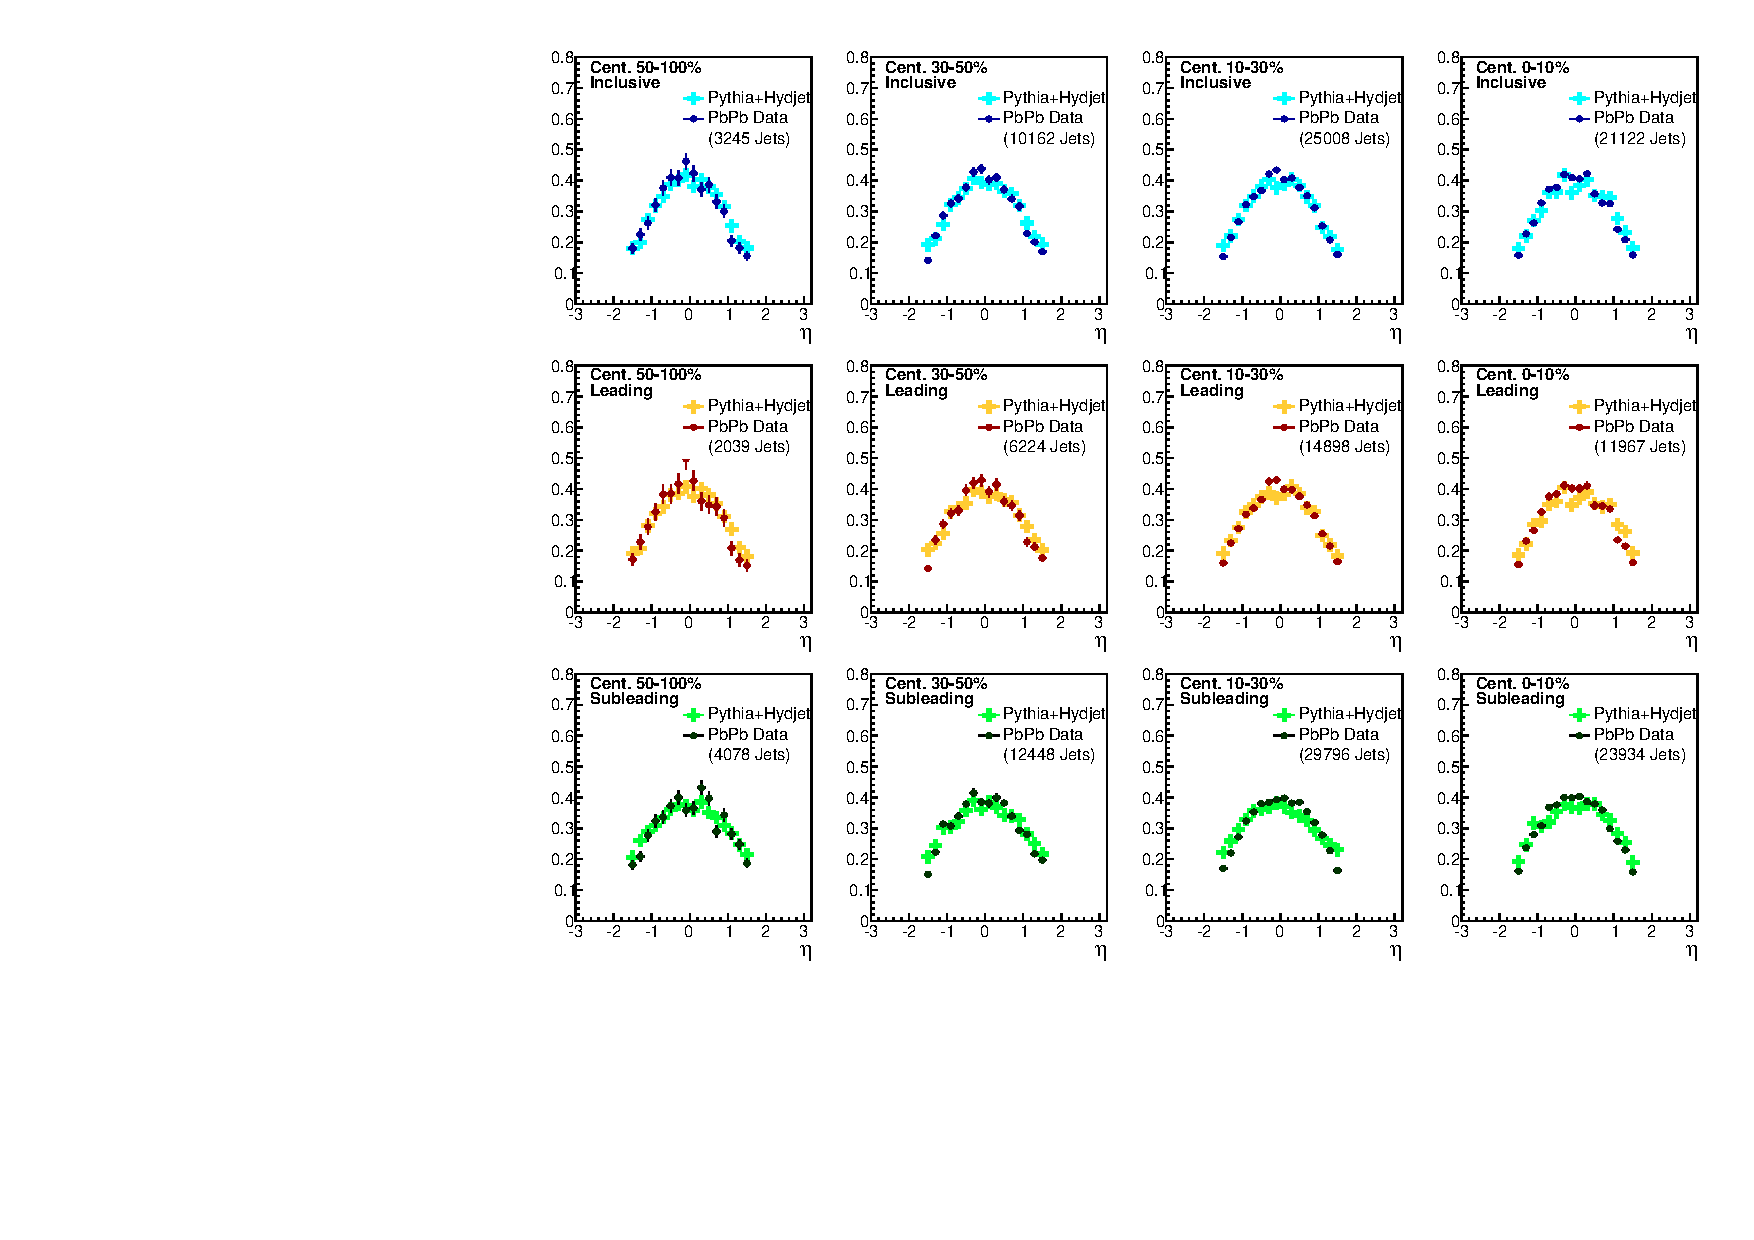
\includegraphics[width=1\textwidth]{figures/Appendices/JetEta_MC_Data_HydJet_RecoJet_JetEtaCut16.pdf}
 \caption{ Pseudorapidity distribution of all jet selections for PbPb data at 2.76 TeV compared to {\sc pythia+hydjet} simulation.}
  \label{fig:PbPbJetEta}
 \end{center}
 \end{figure}
 
 
 \begin{figure}[h!]
 \begin{center}
 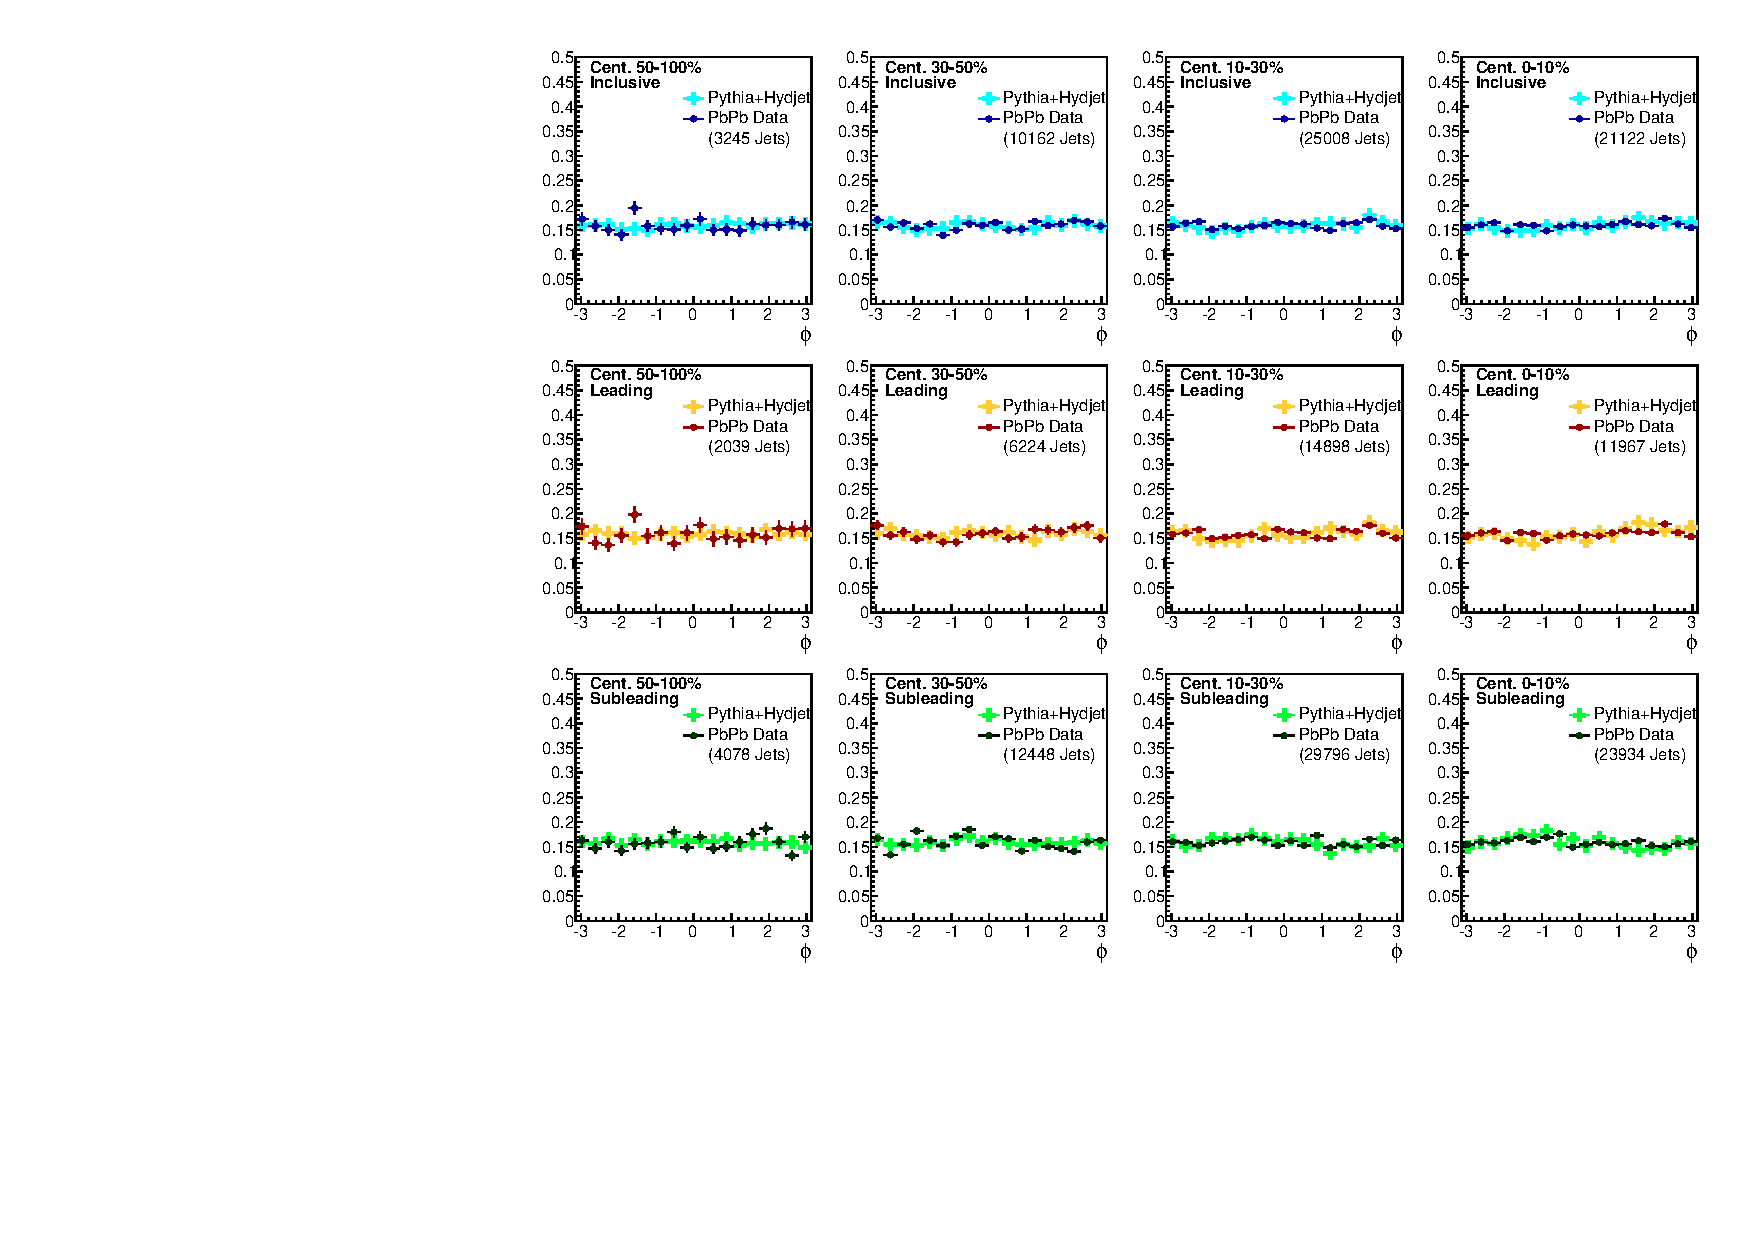
\includegraphics[width=1\textwidth]{figures/Appendices/JetPhi_MC_Data_HydJet_RecoJet_JetEtaCut16.pdf}
 \caption{Azimuthal angle distribution of all jet selections for PbPb data at 2.76 TeV compared to {\sc pythia+hydjet} simulation for each collision centrality bin.}
  \label{fig:PbPbJetPhi}
 \end{center}
 \end{figure}
 

 \clearpage
 
 
 
\subsubsection{Inclusive jet kinematics at 5.02 TeV}
\label{app:kinematics_run2}



Jet $p_{\rm T}$, $\eta$, and $\phi$ distributions for 5.02 TeV data, comparing PbPb data to {\sc pythia+hydjet} and pp data to {\sc pythia} simulation. 


 \begin{figure}[h!]
 \begin{center}

  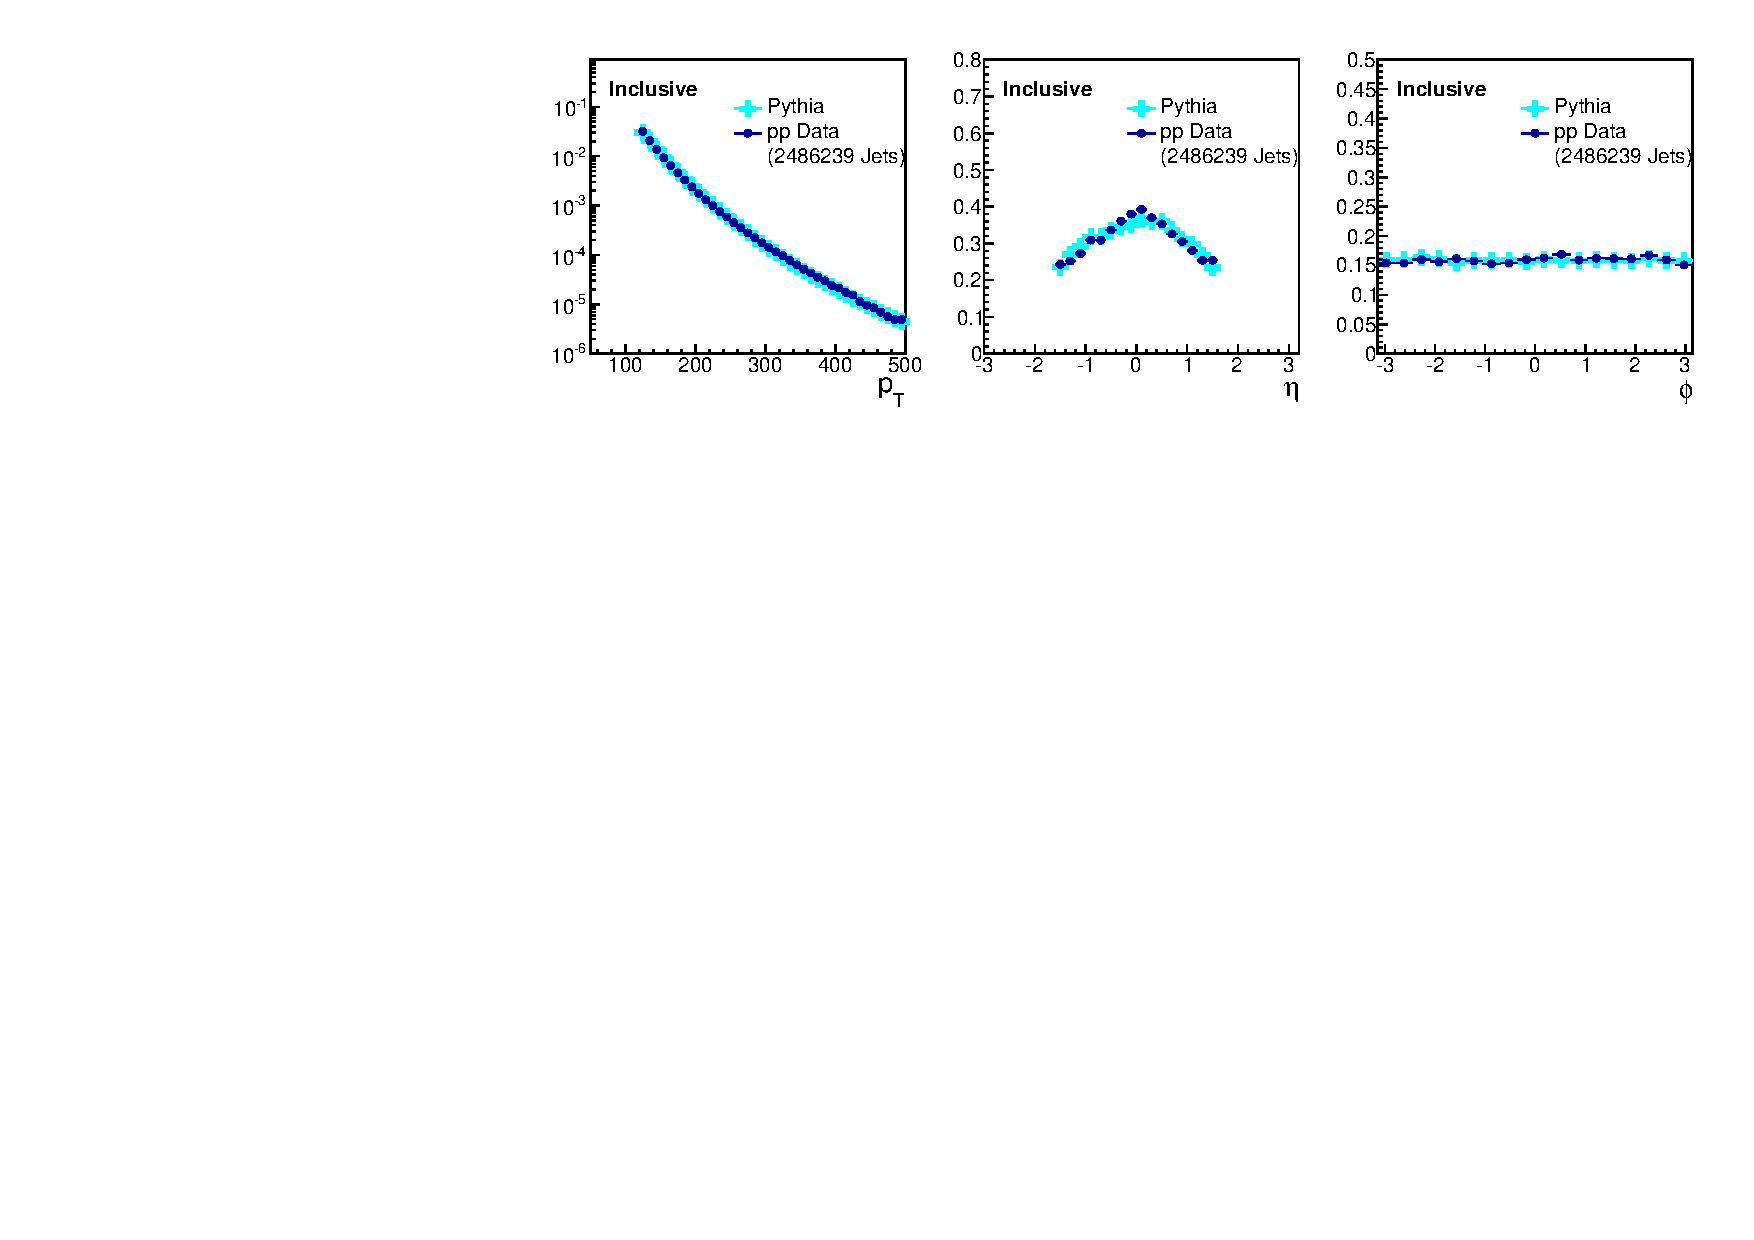
\includegraphics[width=.75\textwidth]{figures/Appendices/JetKinematics_pp_Pythia.pdf}
 \caption{ Distribution of pseudorapidity distribution of all jet selections for PbPb data compared to {\sc pythia+hydjet} simulation for each collision centrality bin.}
\label{fig:ppJetPt2}
 \end{center}
 \end{figure}
 
 
  \begin{figure}[h!]
 \begin{center}
 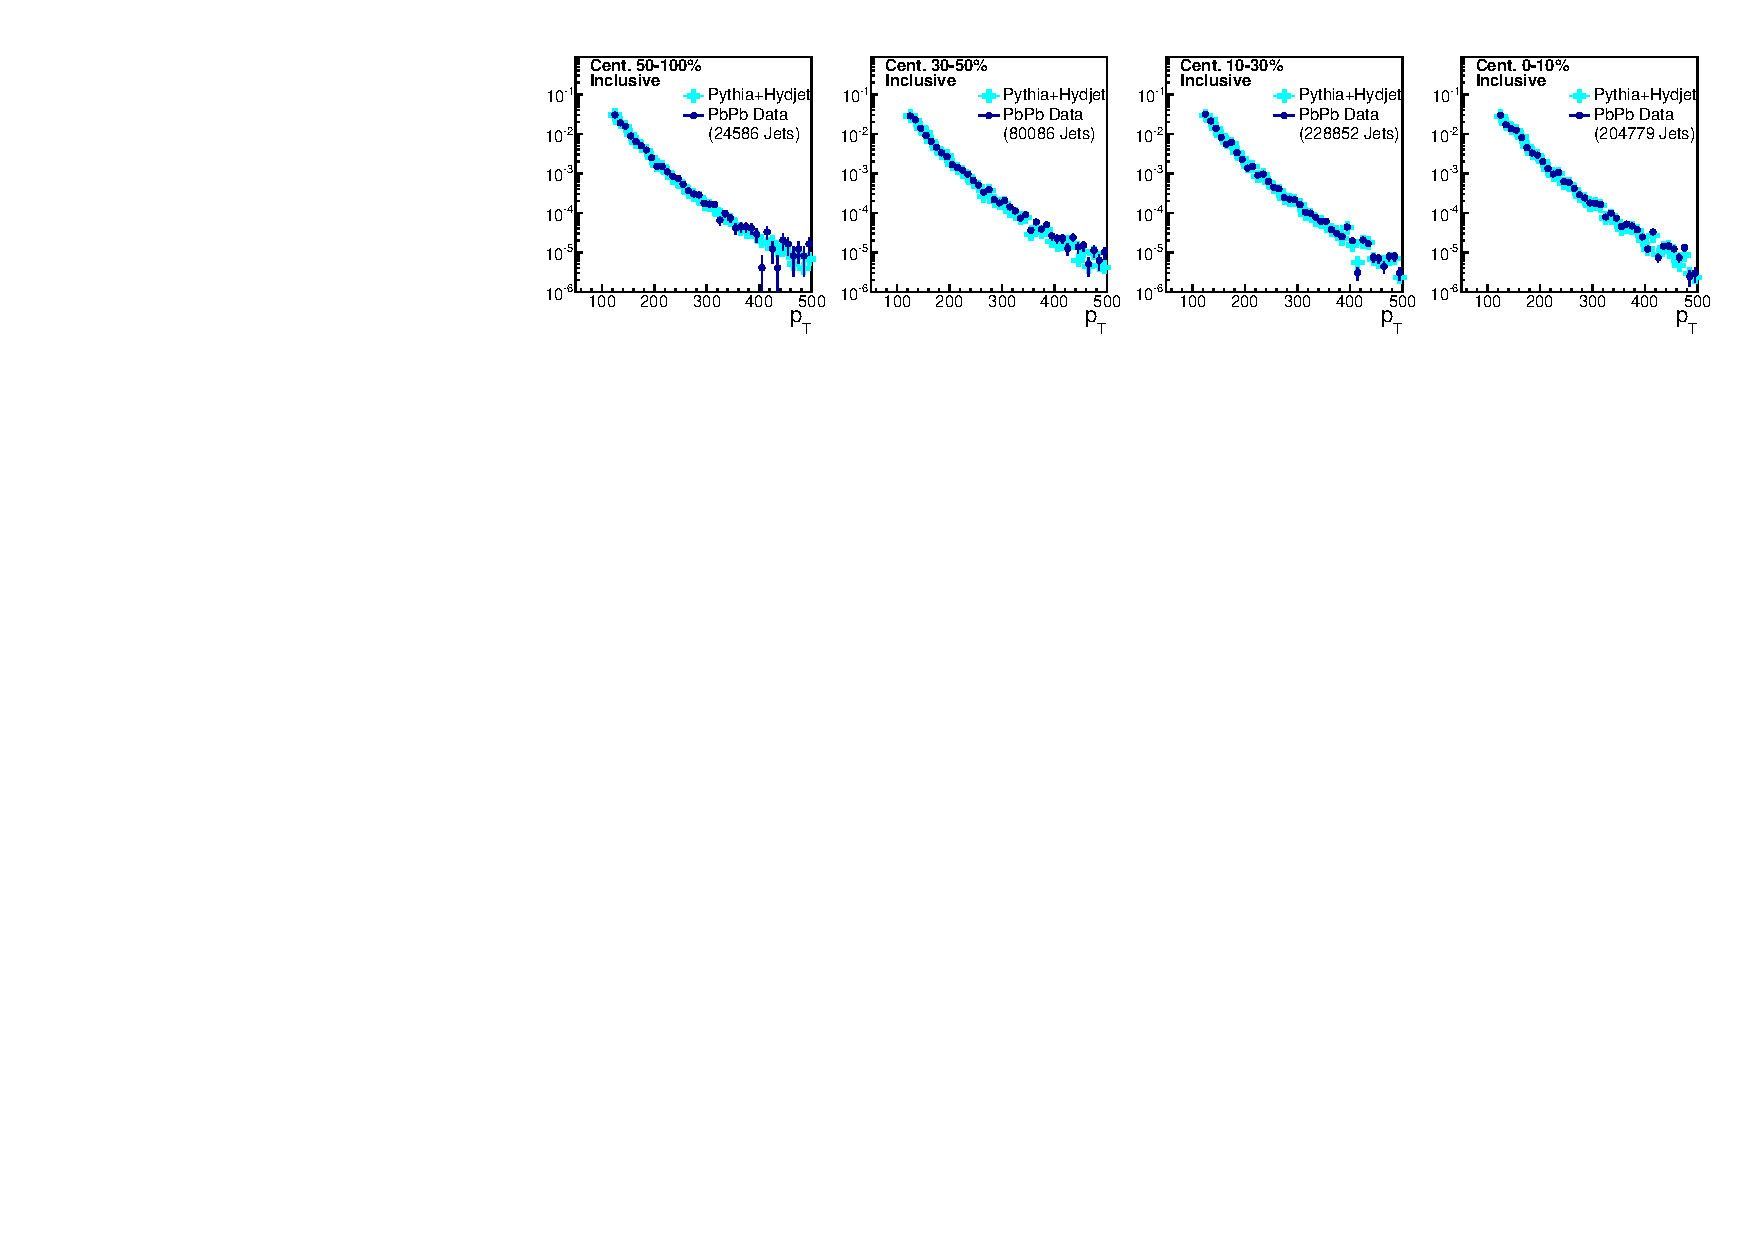
\includegraphics[width=1\textwidth]{figures/Appendices/JetKinematics_PbPb_Hydjet.pdf}
 \caption{Transverse momentum distribution for PbPb data compared to {\sc pythia+hydjet} simulation for each collision centrality bin.}
 \label{fig:PbPbJetPt2} 
 \end{center}
 \end{figure}

  \begin{figure}[h!]
 \begin{center}
 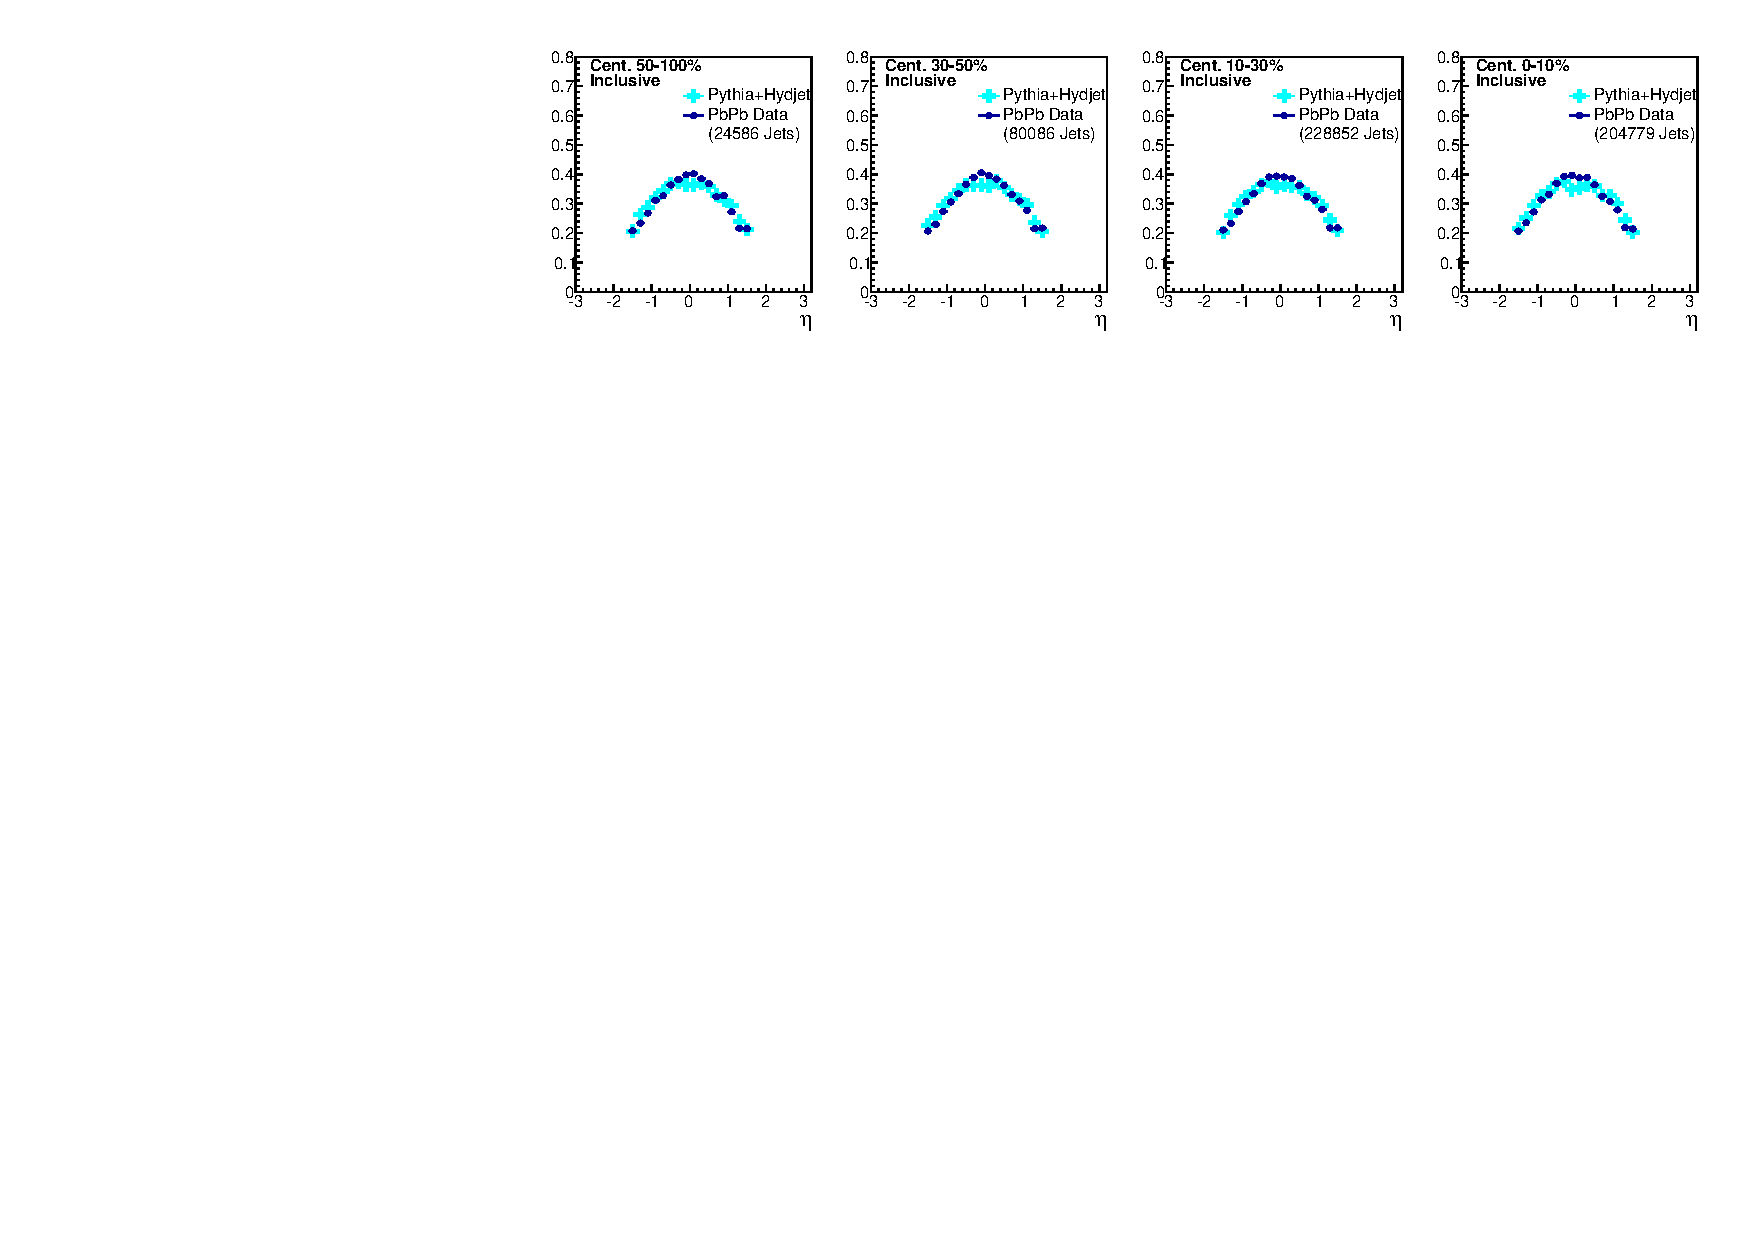
\includegraphics[width=1\textwidth]{figures/Appendices/JetEta_PbPb_Hydjet.pdf}
 \caption{Jet $\eta$ distribution for PbPb data compared to {\sc pythia+hydjet} simulation for each collision centrality bin.}
 \label{fig:PbPbJetEta2} 
 \end{center}
 \end{figure}

 
  \begin{figure}[h!]
 \begin{center}
 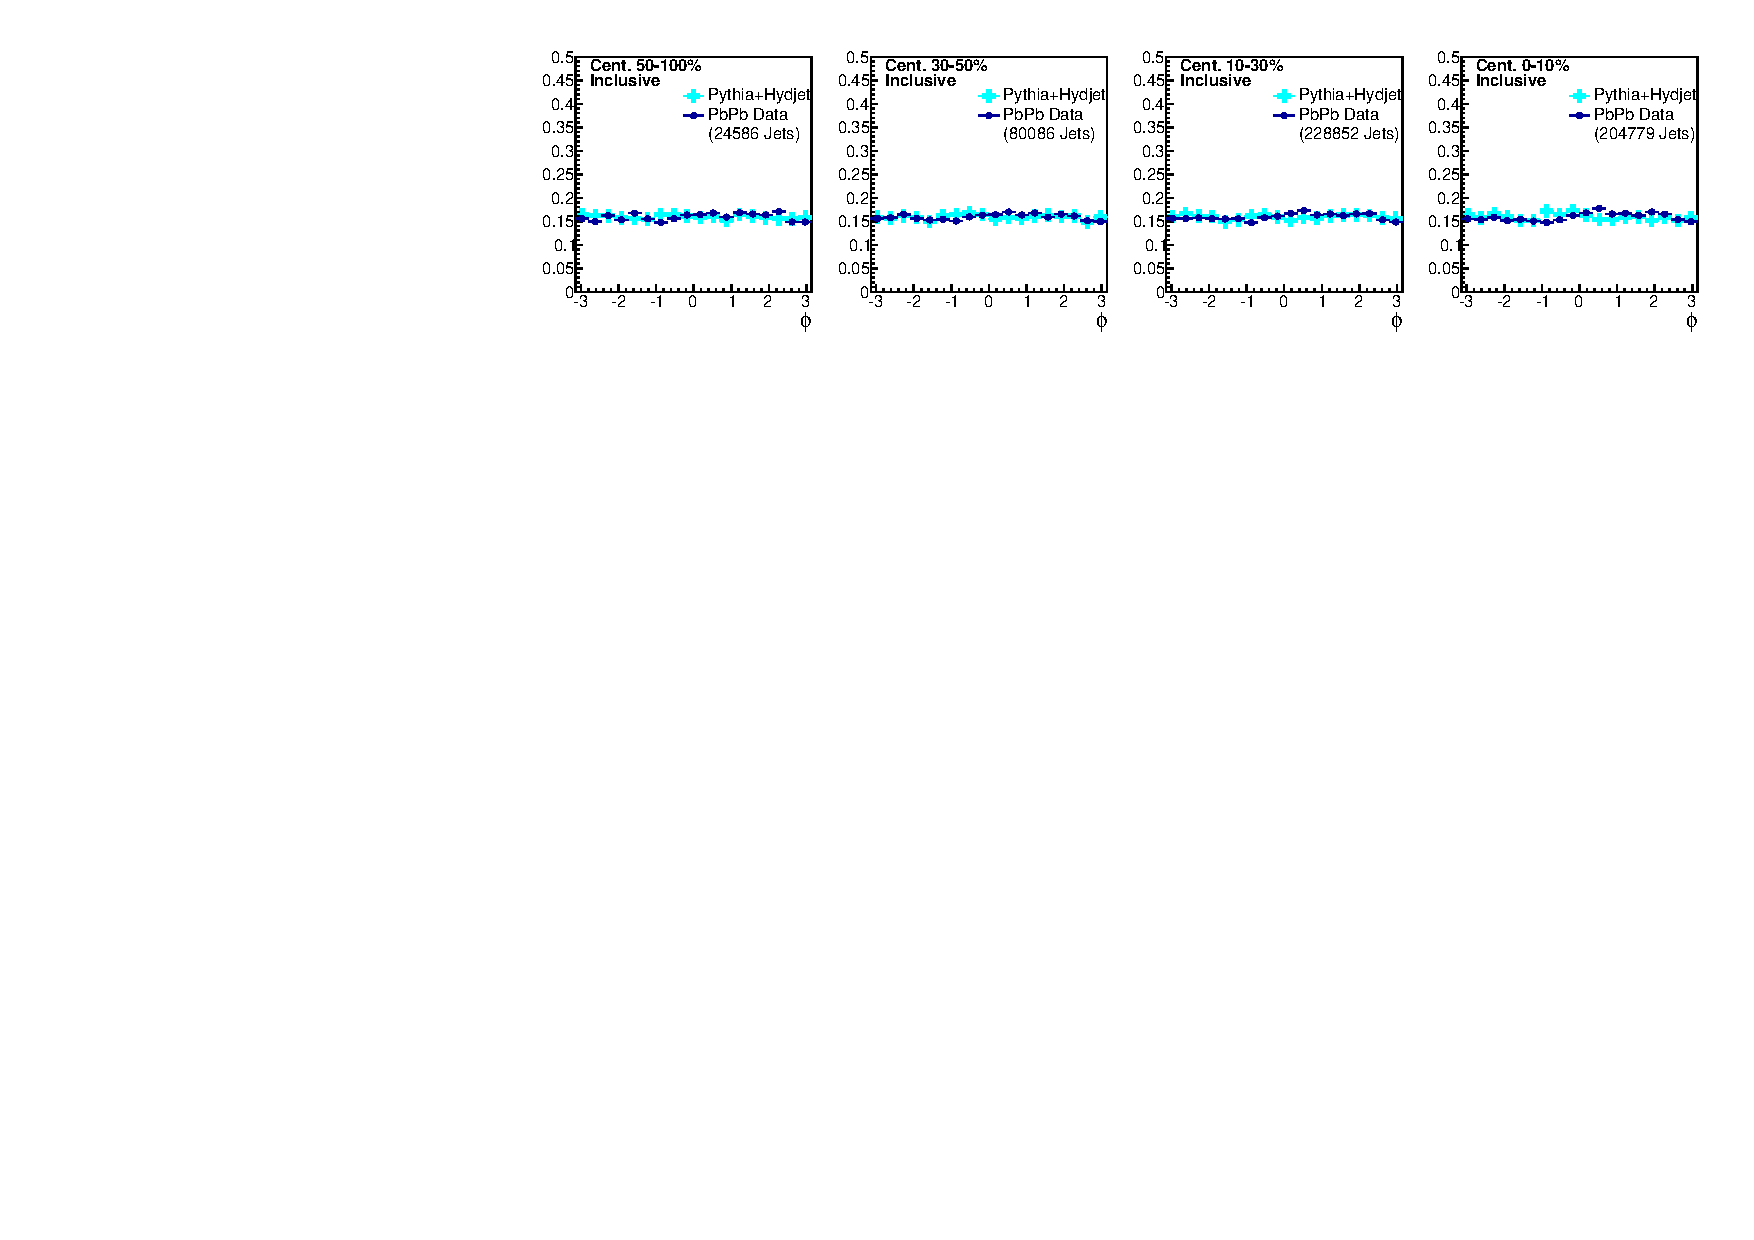
\includegraphics[width=1\textwidth]{figures/Appendices/JetPhi_PbPb_Hydjet.pdf}
 \caption{Jet $\phi$ distribution for PbPb data compared to {\sc pythia+hydjet} simulation for each collision centrality bin.}
 \label{fig:PbPbJetPhi2} 
 \end{center}
 \end{figure}

  
 \subsubsection{Dijet kinematics in asymmetry classes at 2.76 TeV}

In the figures below, jet transverse momentum, pseudorapidity, and azimuth are shown for our Aj-inclusive sample, compared to each Aj selection in our analysis.  Note that $A_{\rm J}$-selection primarily affects the subleading jet spectrum, while the leading jet spectrum is nearly unchanged.  Jet $\eta$ and jet $\phi$ exhibit no significant $A_{\rm J}$-dependence for leading or subleading jets.  Distributions are shown first for pp, and then for PbPb data at 2.76 TeV.








\begin{figure}[htbp]
\begin{center}
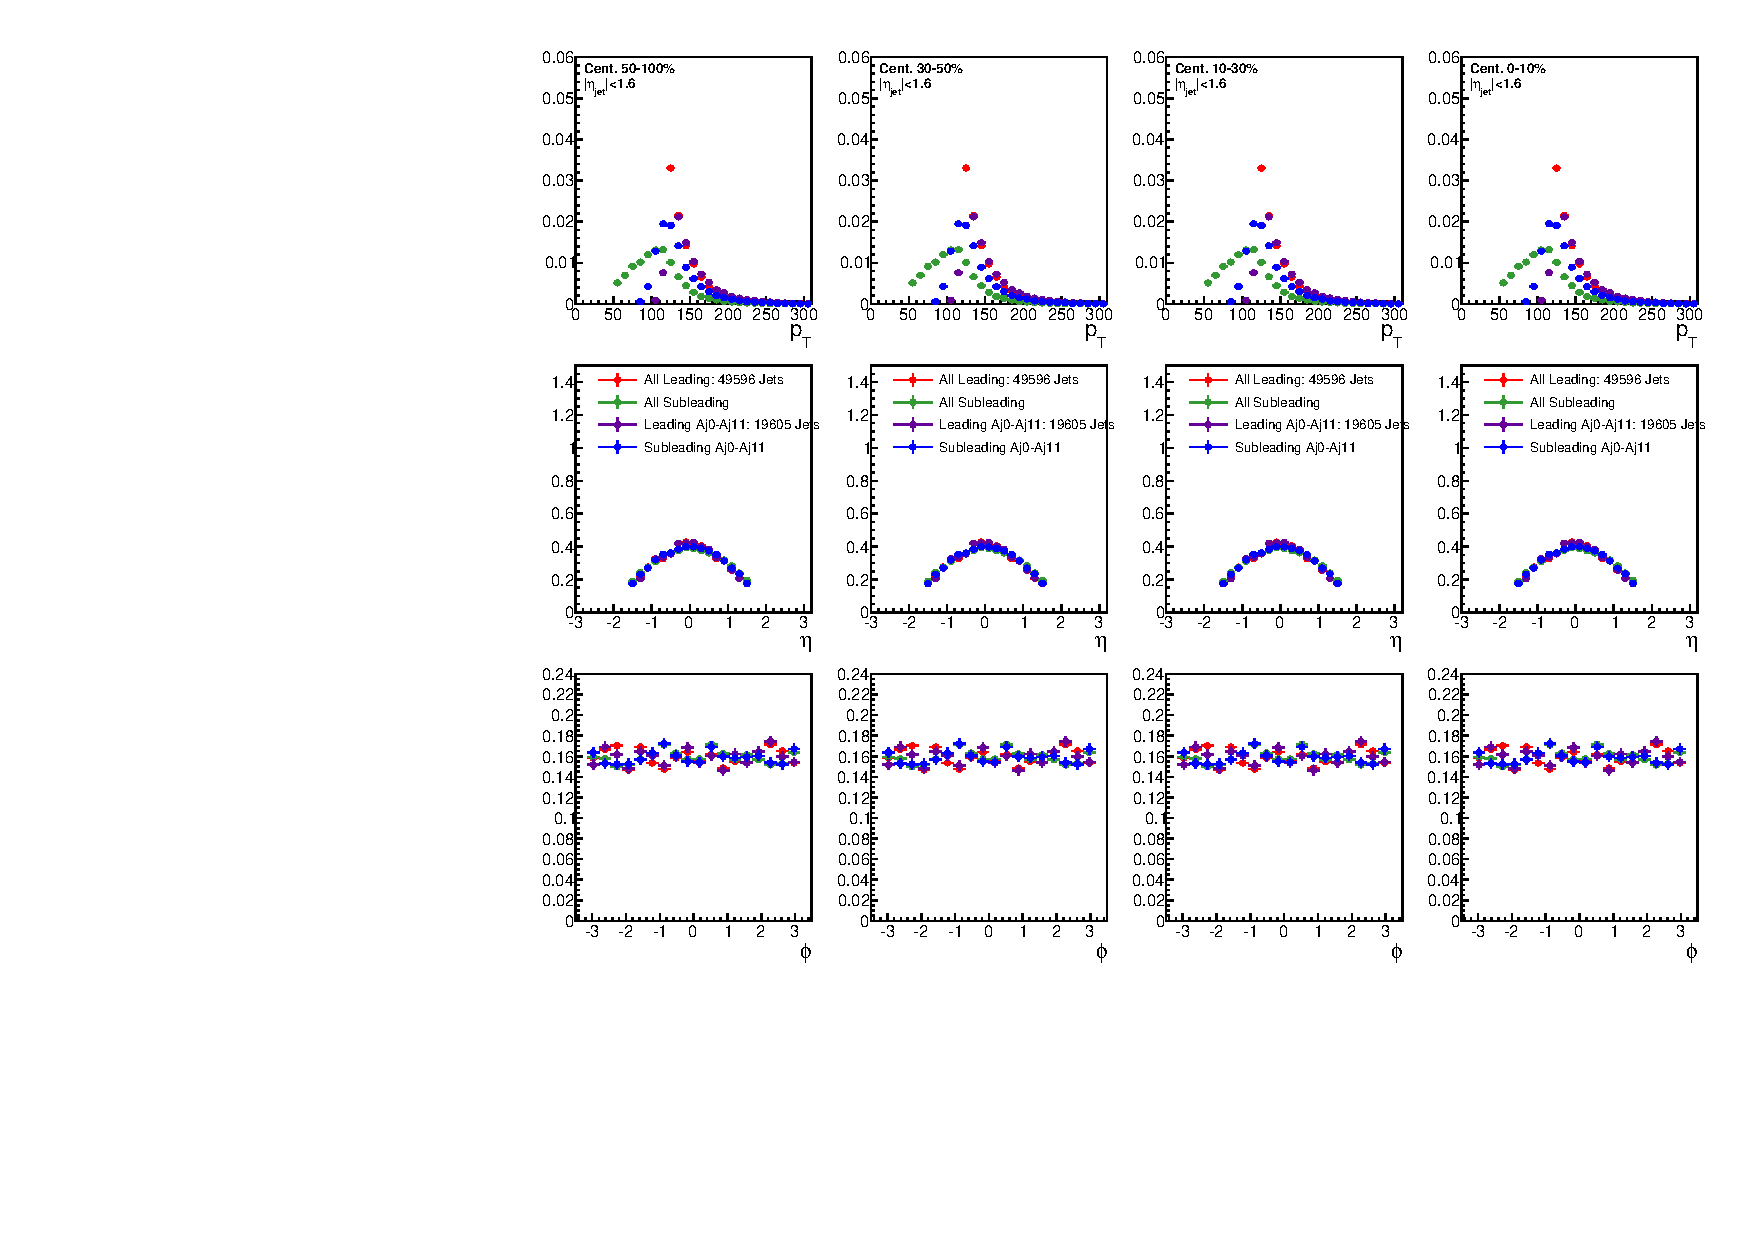
\includegraphics[width=0.99\textwidth]{figures/Appendices/JetSummary_pp_Aj0_Aj11.pdf}
\caption{
Jet $p_{\rm T}$, $\eta$, and $\phi$ for all  pp dijets and for  pp dijets with $A_{\rm J}$:  $0<A_{\rm J}<0.11$.  
}
\label{fig:JetKin ppAj0Aj11}
\end{center}
\end{figure}

\begin{figure}[htbp]
\begin{center}
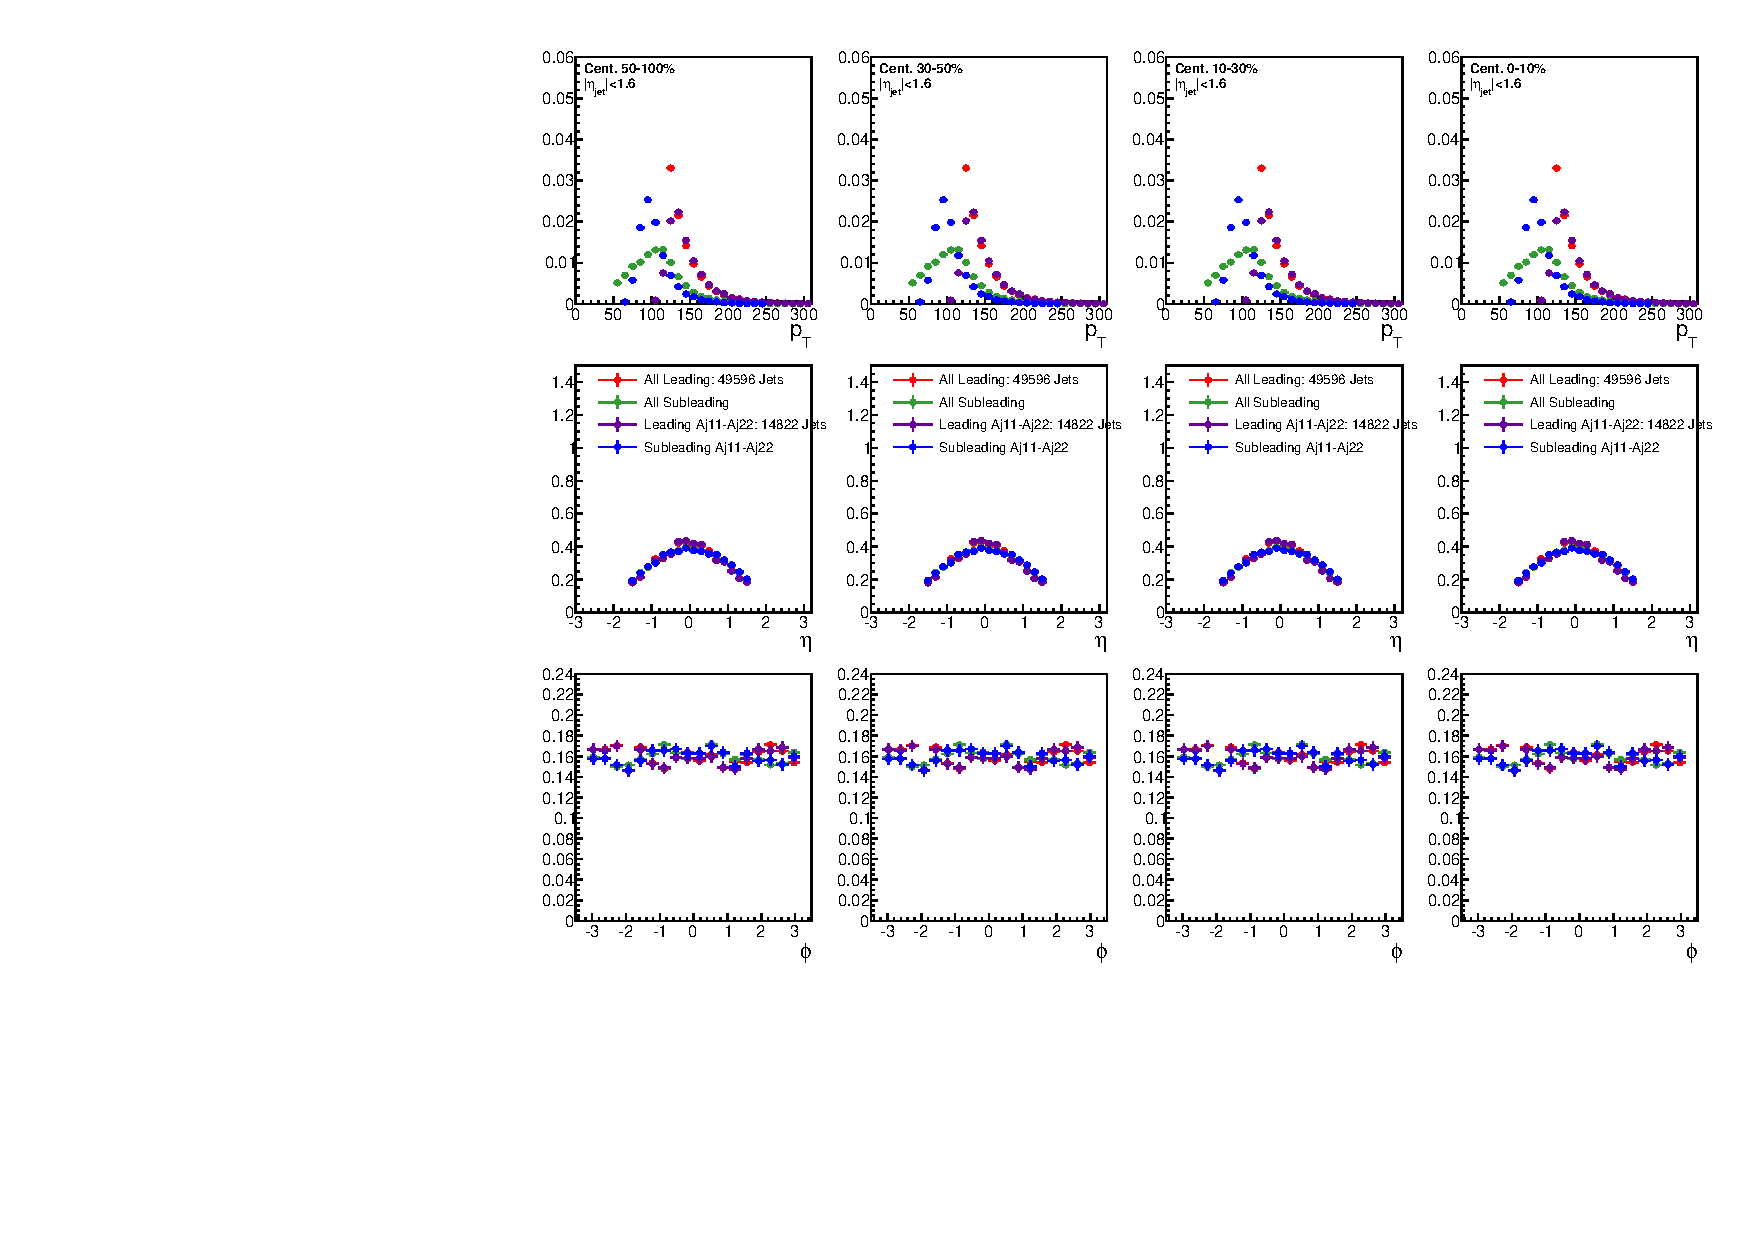
\includegraphics[width=0.99\textwidth]{figures/Appendices/JetSummary_pp_Aj11_Aj22.pdf}
\caption{
Jet $p_{\rm T}$, $\eta$, and $\phi$ for all  pp dijets and for  pp dijets with $A_{\rm J}$:  $0.11<A_{\rm J}<0.22$.  
}
\label{fig:JetKin ppAj11Aj22}
\end{center}
\end{figure}

\begin{figure}[htbp]
\begin{center}
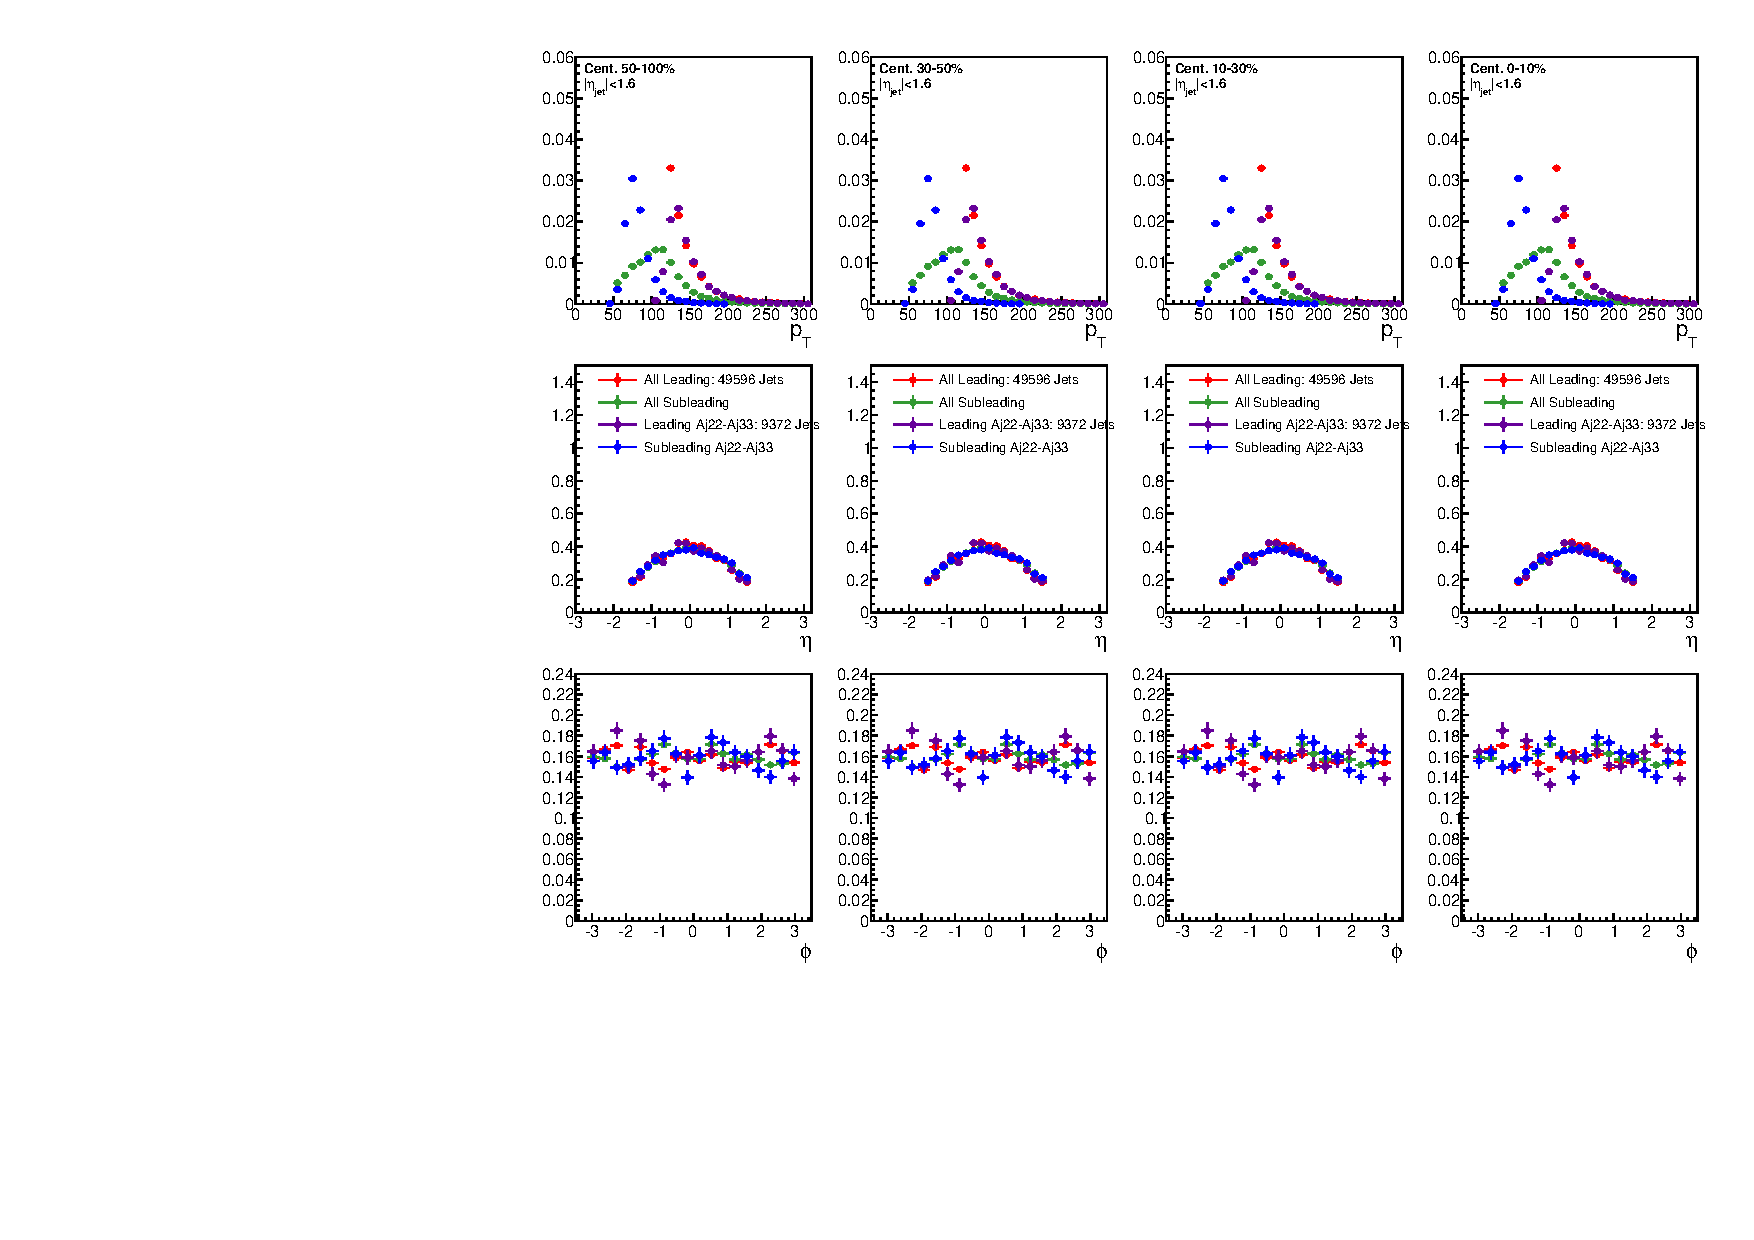
\includegraphics[width=0.99\textwidth]{figures/Appendices/JetSummary_pp_Aj22_Aj33.pdf}
\caption{
Jet $p_{\rm T}$, $\eta$, and $\phi$ for all  pp dijets and for  pp dijets with $A_{\rm J}$:  $0.22<A_{\rm J}<0.33$.  
}
\label{fig:JetKin ppAj22Aj33}
\end{center}
\end{figure}


\begin{figure}[htbp]
\begin{center}
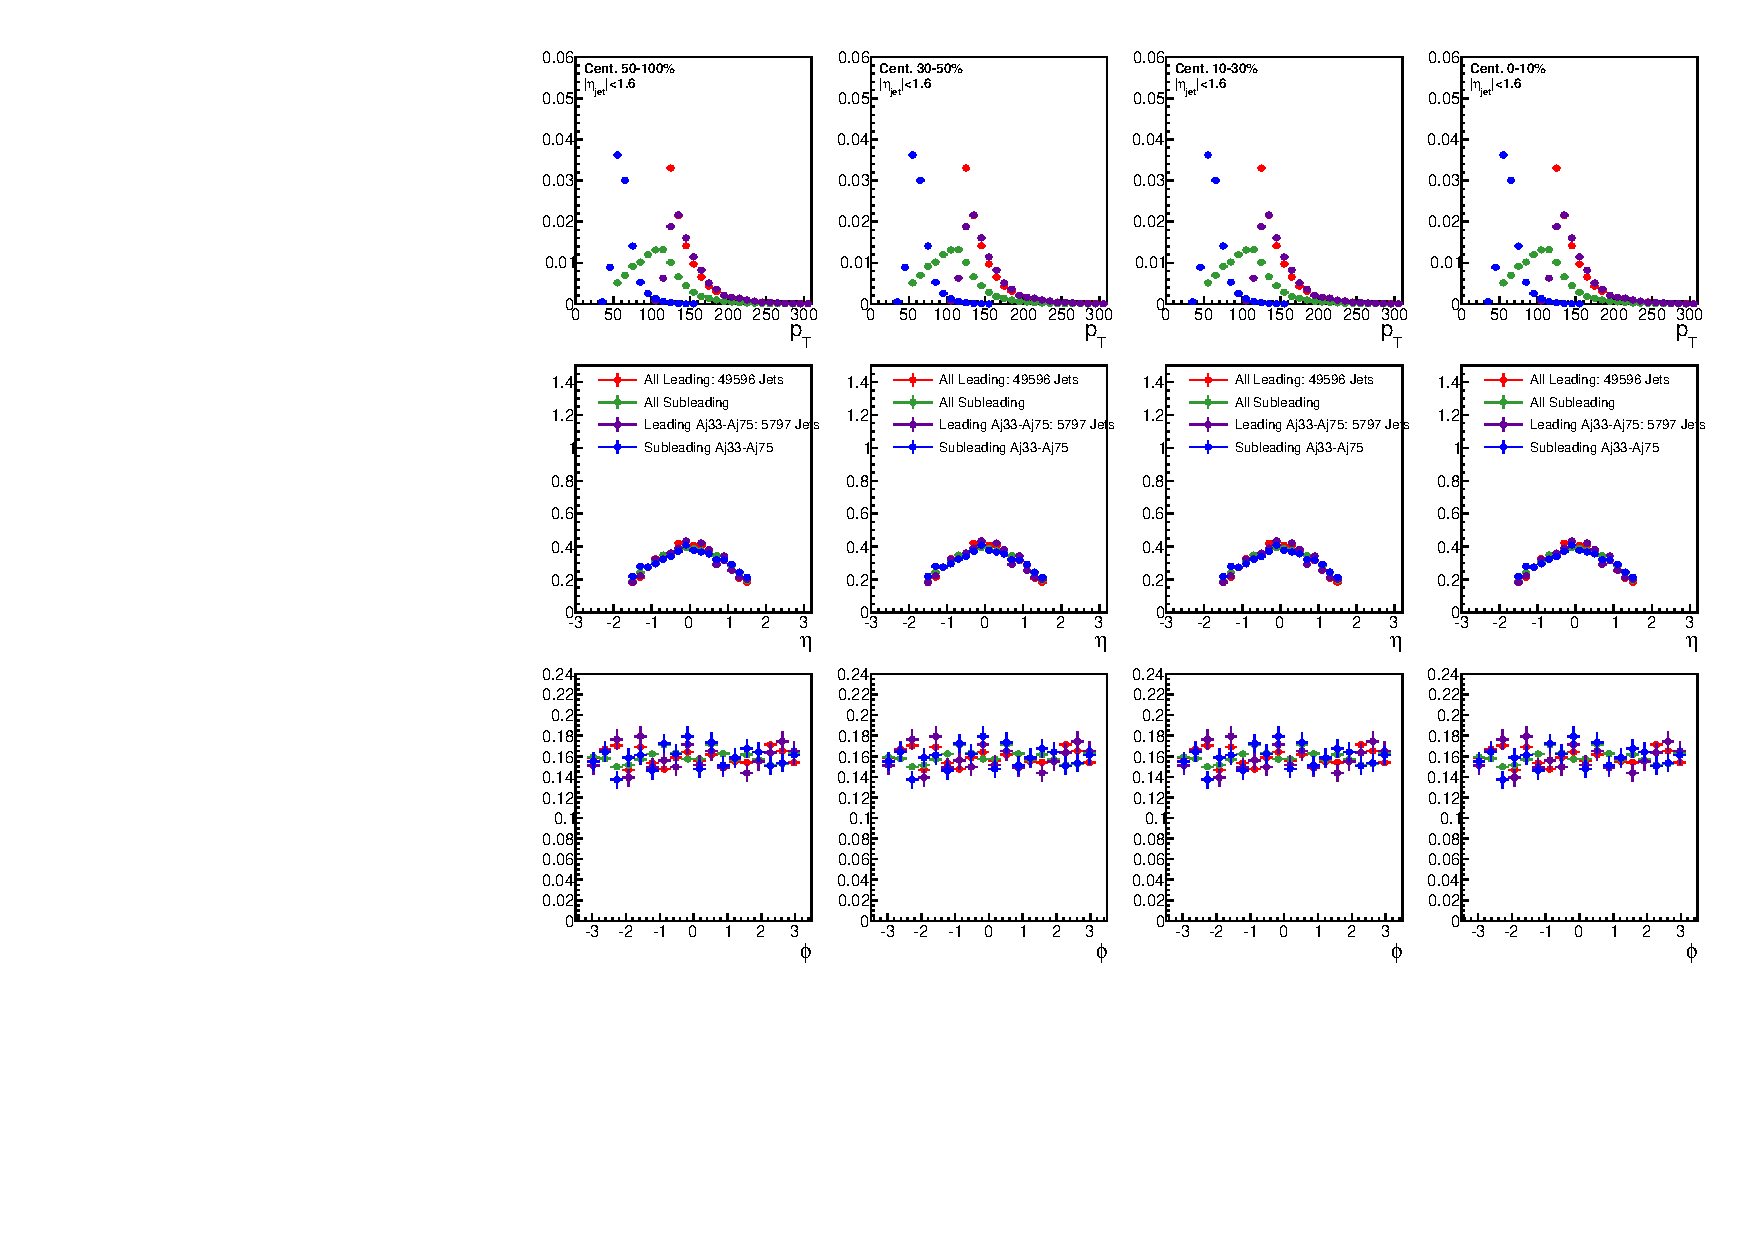
\includegraphics[width=0.99\textwidth]{figures/Appendices/JetSummary_pp_Aj33_Aj75.pdf}
\caption{
Jet $p_{\rm T}$, $\eta$, and $\phi$ for all  pp dijets and for  pp dijets with $A_{\rm J}$:  $A_{\rm J}>0.33$.  
}
\label{fig:JetKinppAj33Aj75}
\end{center}
\end{figure}


\begin{figure}[htbp]
\begin{center}
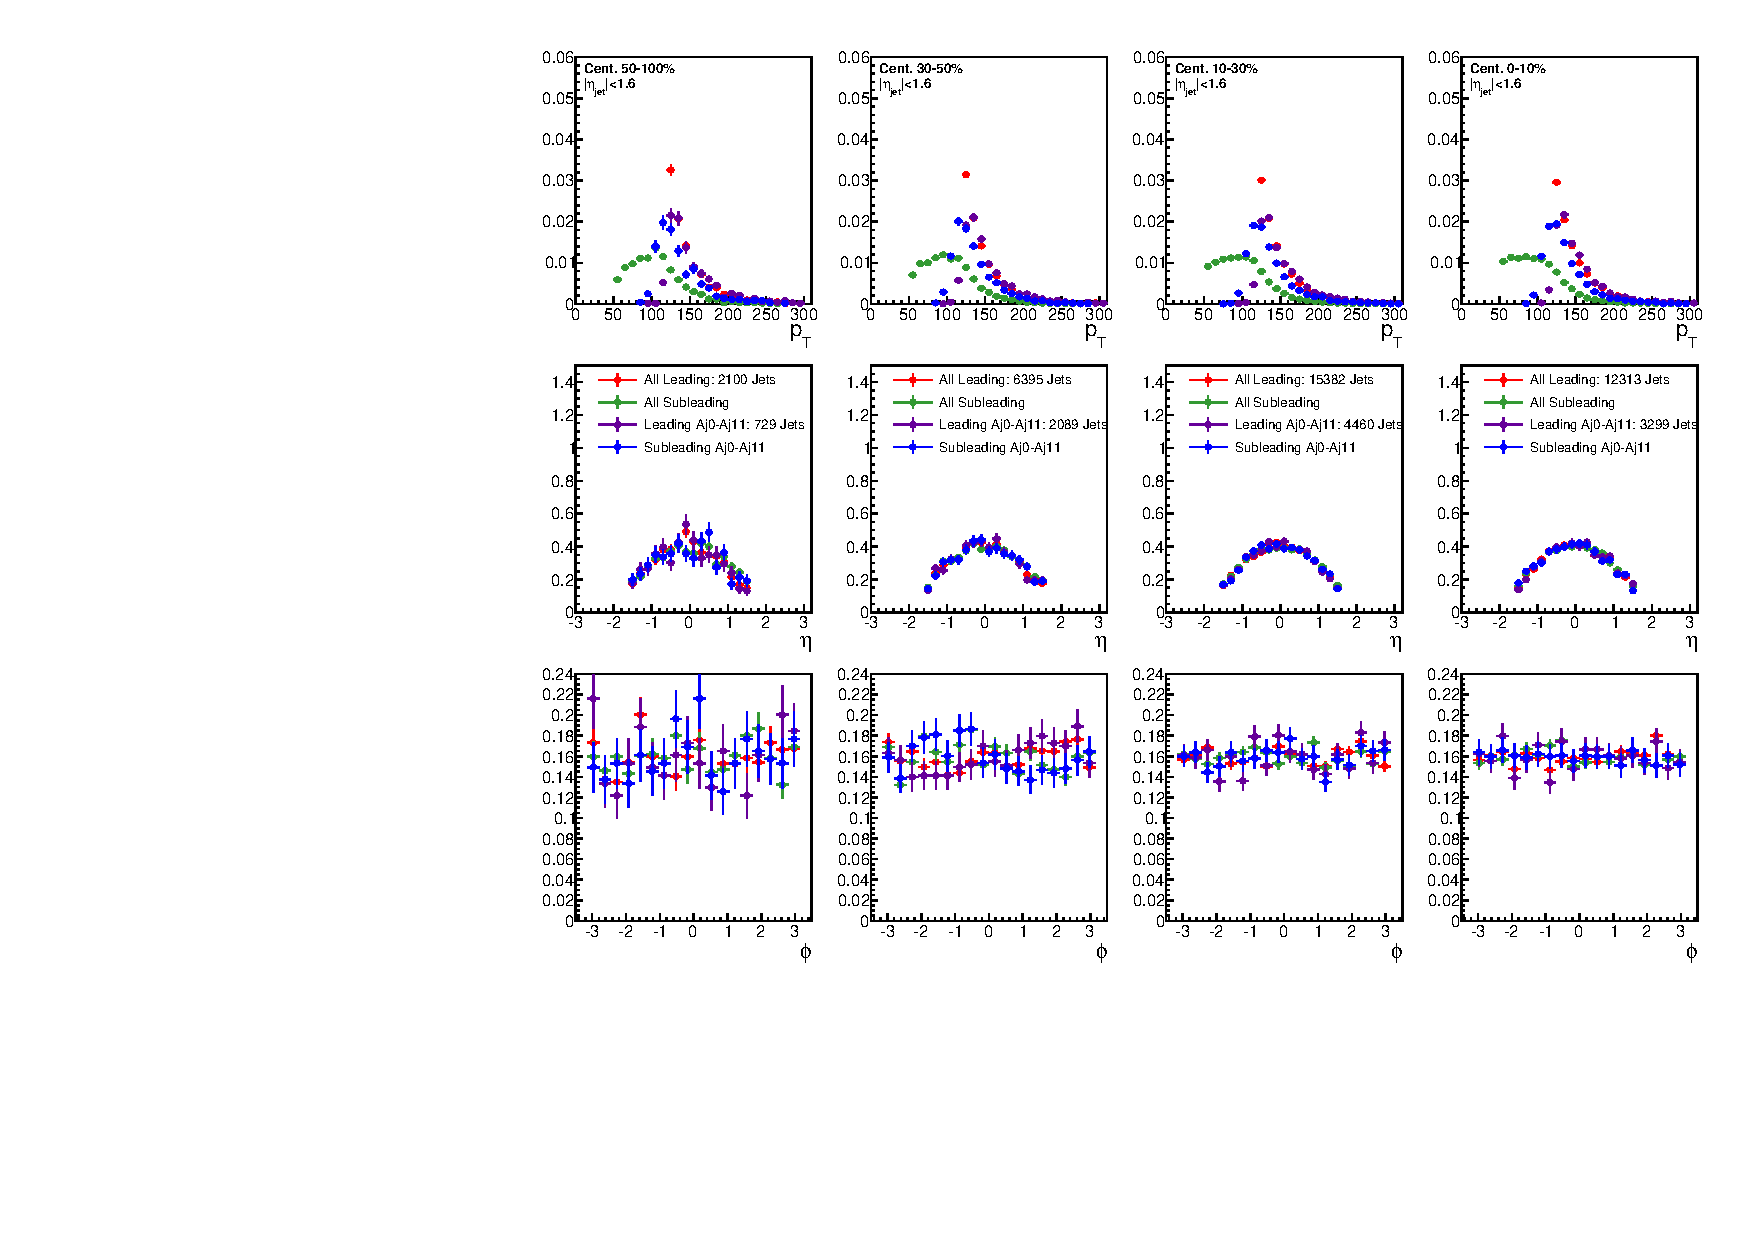
\includegraphics[width=0.99\textwidth]{figures/Appendices/JetSummary_PbPb_Aj0_Aj11.pdf}
\caption{Jet $p_{\rm T}$, $\eta$, and $\phi$ for all PbPb dijets and for PbPb dijets with  $0<A_{\rm J}<0.11$.  
}
\label{fig:JetKinPbPbAj0Aj11}
\end{center}
\end{figure}

\begin{figure}[htbp]
\begin{center}
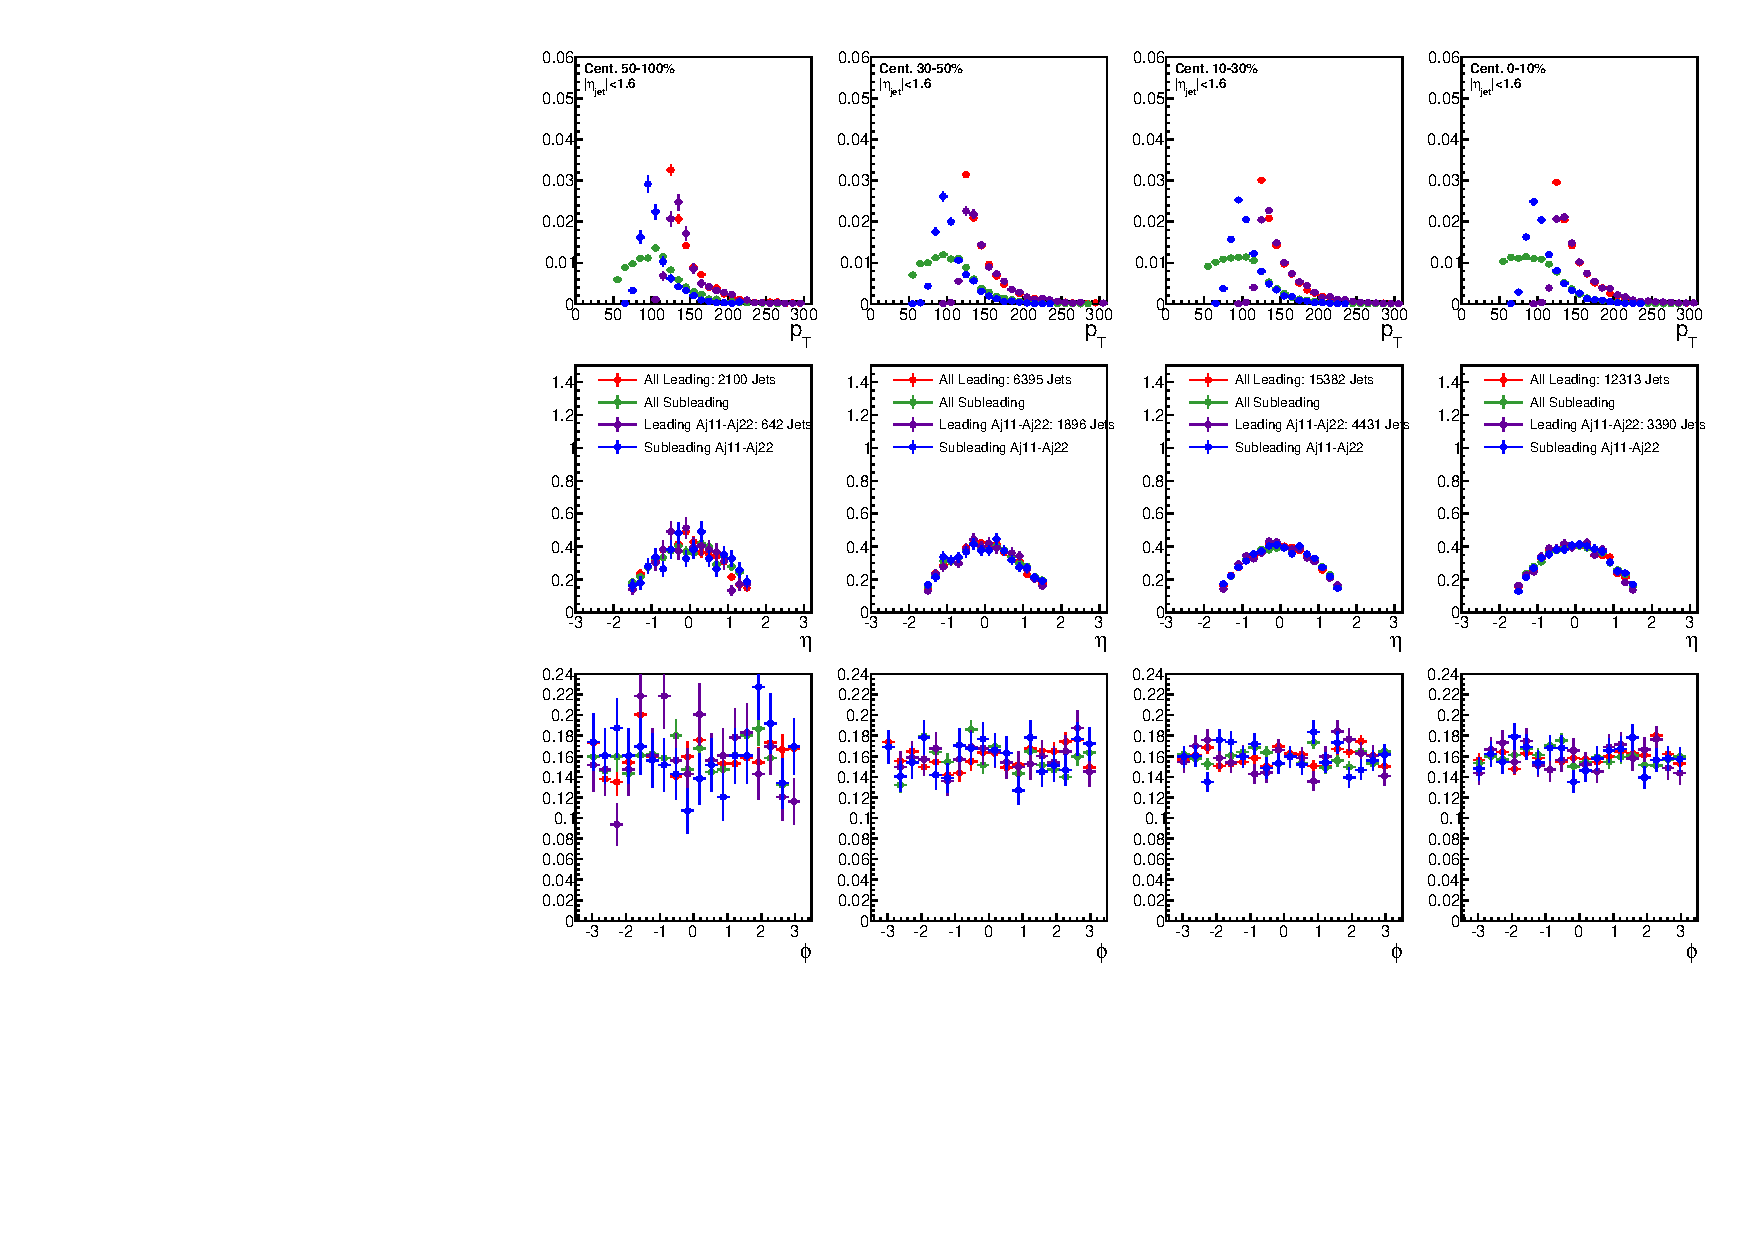
\includegraphics[width=0.99\textwidth]{figures/Appendices/JetSummary_PbPb_Aj11_Aj22.pdf}
\caption{
Jet $p_{\rm T}$, $\eta$, and $\phi$ for all PbPb dijets and for PbPb dijets with $0.11<A_{\rm J}<0.22$.  
}
\label{fig:JetKinPbPbAj11Aj22}
\end{center}
\end{figure}

\begin{figure}[htbp]
\begin{center}
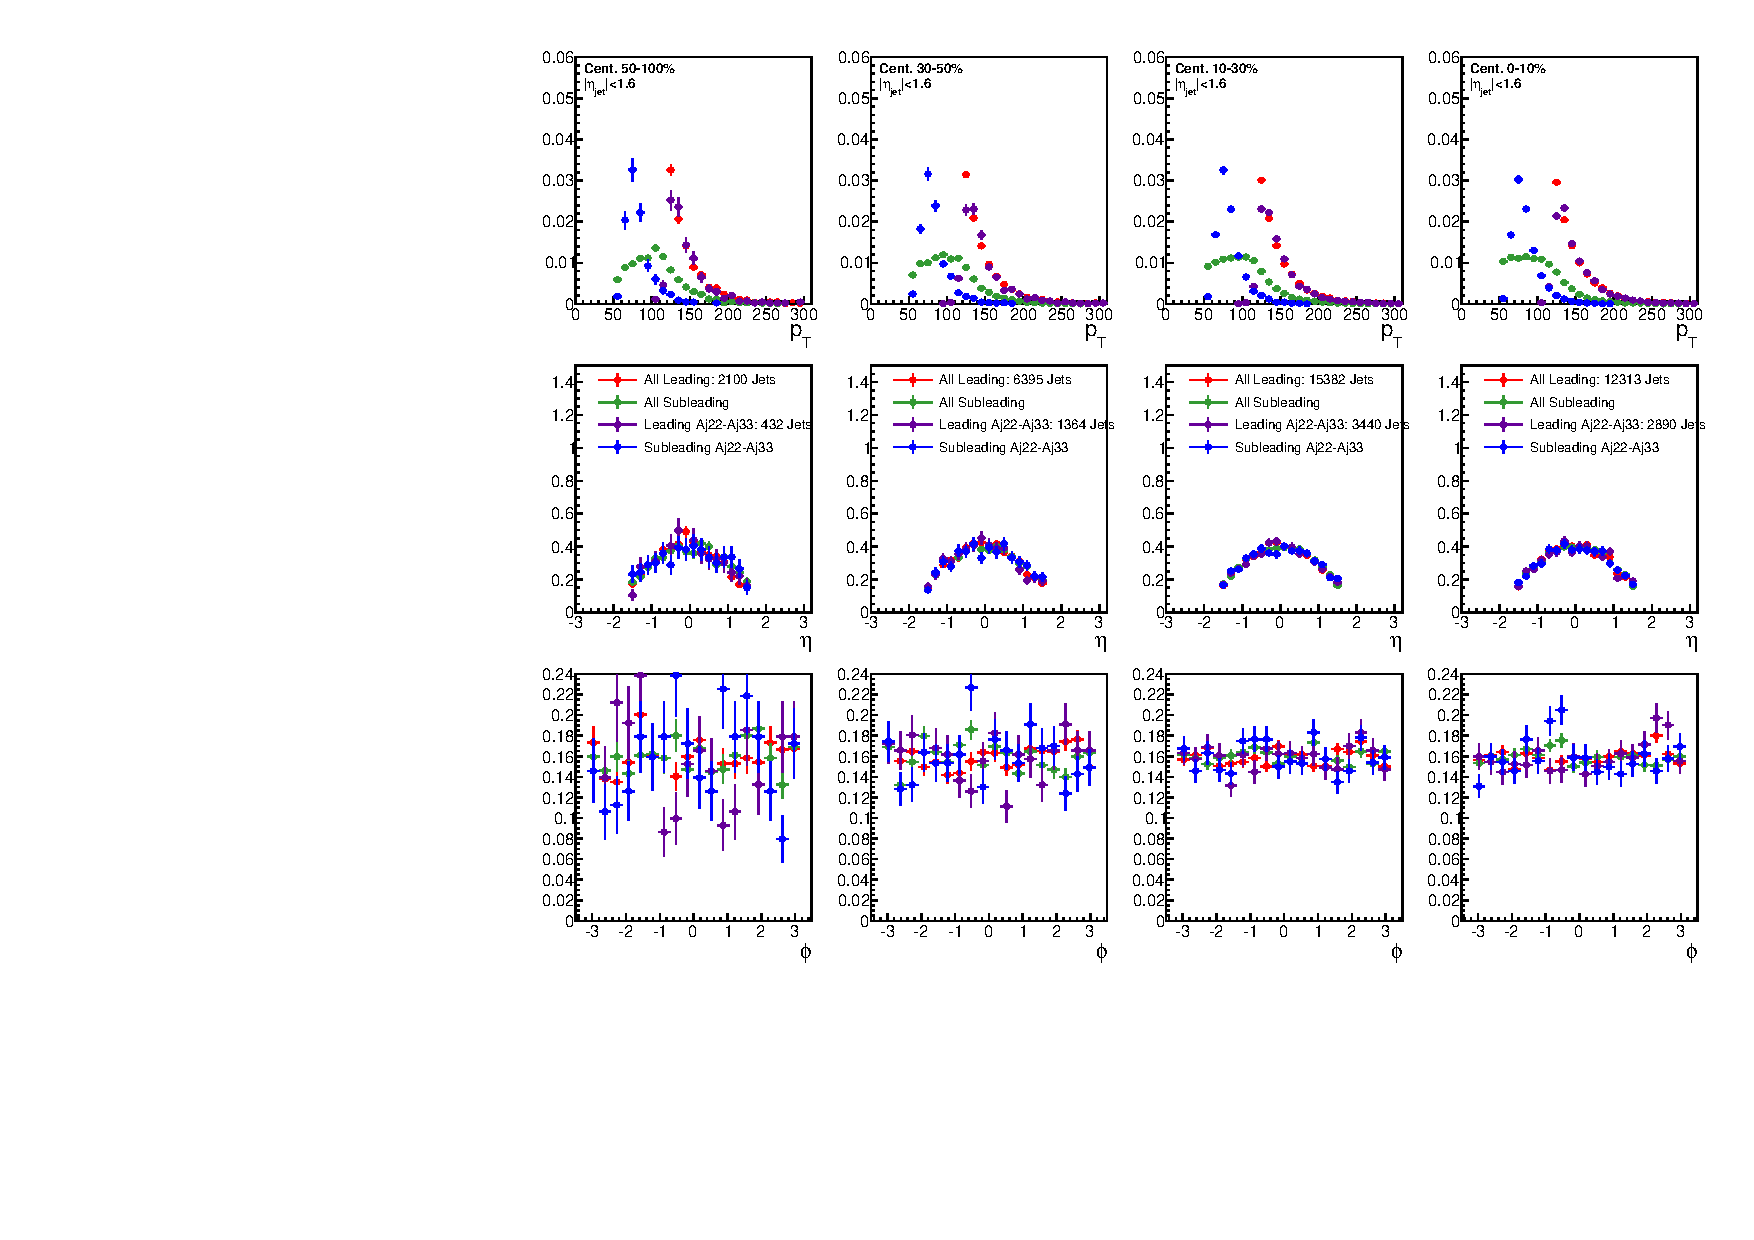
\includegraphics[width=0.99\textwidth]{figures/Appendices/JetSummary_PbPb_Aj22_Aj33.pdf}
\caption{
Jet $p_{\rm T}$, $\eta$, and $\phi$ for all PbPb dijets and for PbPb dijets with $0.22<A_{\rm J}<0.33$.  
}
\label{fig:JetKinPbPbAj22Aj33}
\end{center}
\end{figure}


\begin{figure}[htbp]
\begin{center}
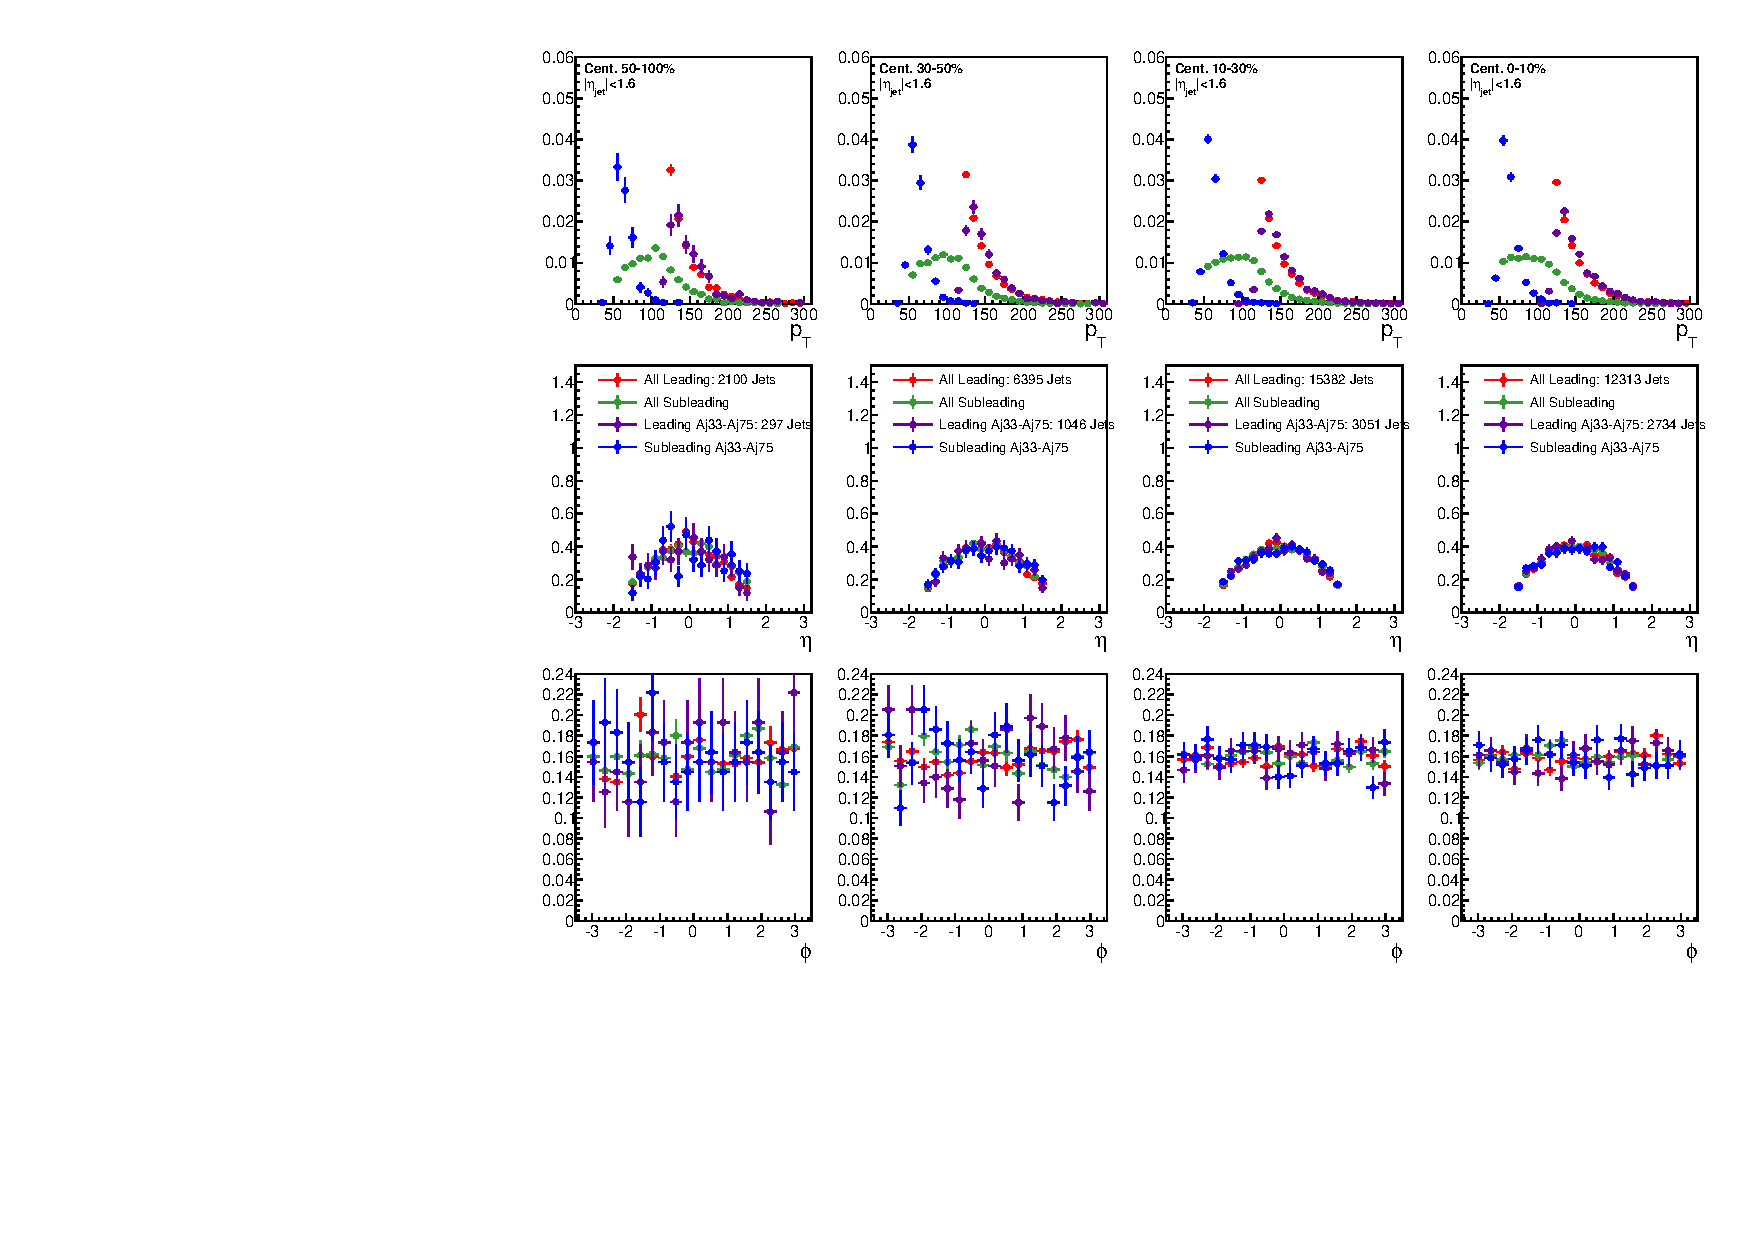
\includegraphics[width=0.99\textwidth]{figures/Appendices/JetSummary_PbPb_Aj33_Aj75.pdf}
\caption{
Jet $p_{\rm T}$, $\eta$, and $\phi$ for all PbPb dijets and for PbPb dijets with $A_{\rm J}>0.33$.  
}
\label{fig:JetKinPbPbAj33Aj75}
\end{center}
\end{figure}


\clearpage




\subsection{Background fitting details}

\label{app:bkg_fits}

Figures~\ref{fig:dijet_fit}-\ref{fig:inc_fit} show the two steps of fits involved in modeling the the background distribution in $\Delta\phi$, as discussed in section~\ref{sec:bkg_sub}.

\begin{figure}[h!]
\begin{center}
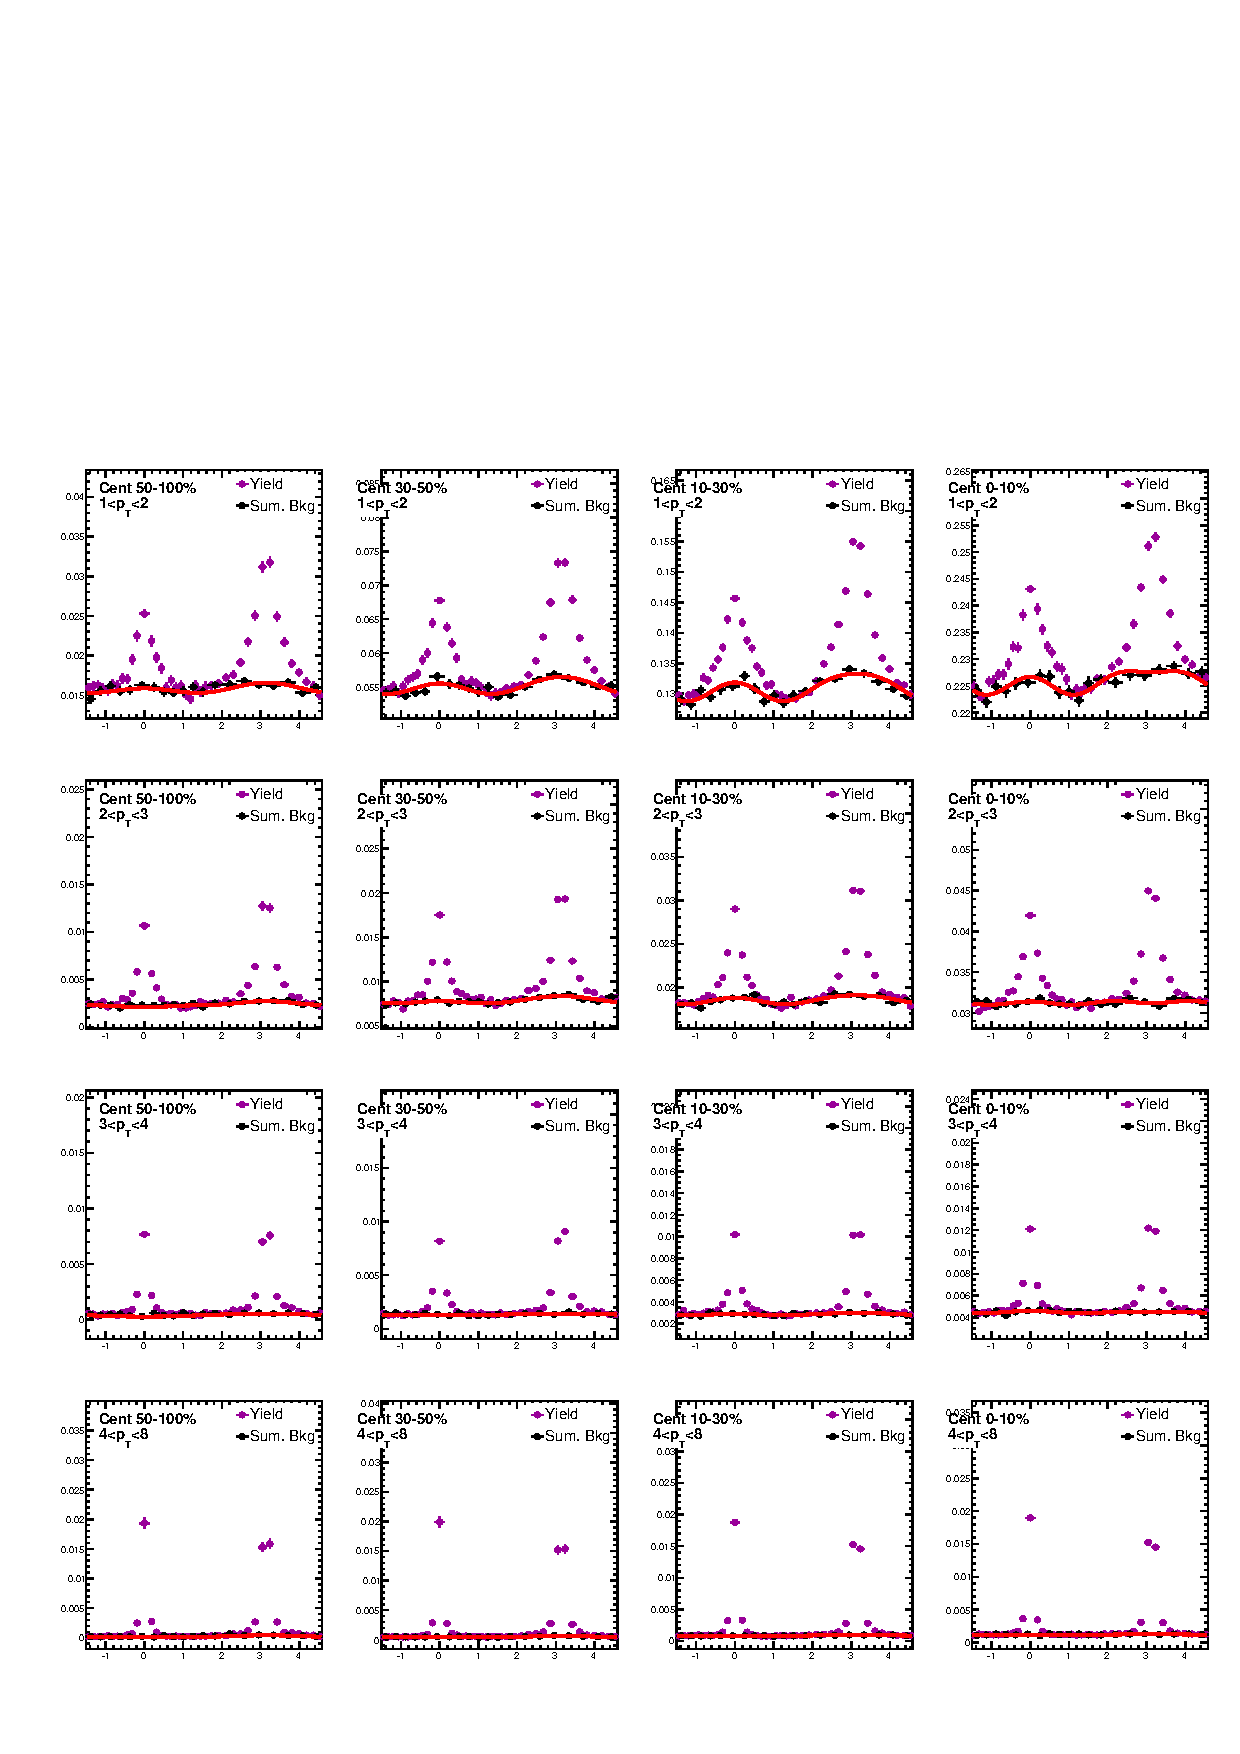
\includegraphics[width=0.9\textwidth]{figures/Appendices/DijetFreeFitsGluedBackgroundV1V2V3.pdf}
\caption[Dijet background fits (preliminary step)]{Dijet combined background $\Delta\phi$ distributions, estimated by projection over the region 1.5$<|\Delta\eta|<$3.0.  Here the ''near-side'' region $\frac{-\pi}{2}<\Delta\phi<\frac{\pi}{2}$ is taken from the leading jet correlation, while the ''away-side'' $\frac{-\pi}{2}<\Delta\phi<\frac{\pi}{2}$ is taken from the subleading jet correlation.  The resulting combined background distribution is fit with the function $B^{dijet}(\Delta\phi) = B_{0}(1+2\rm{V}_{1}$Cos($\Delta\phi$)+$2\rm{V}_{2}$Cos(2$\Delta\phi$))+$2\rm{V}_{3}$Cos(3$\Delta\phi$)).}
\label{fig:dijet_fit}
\end{center}
\end{figure}


\begin{figure}[hbtp]
\begin{center}
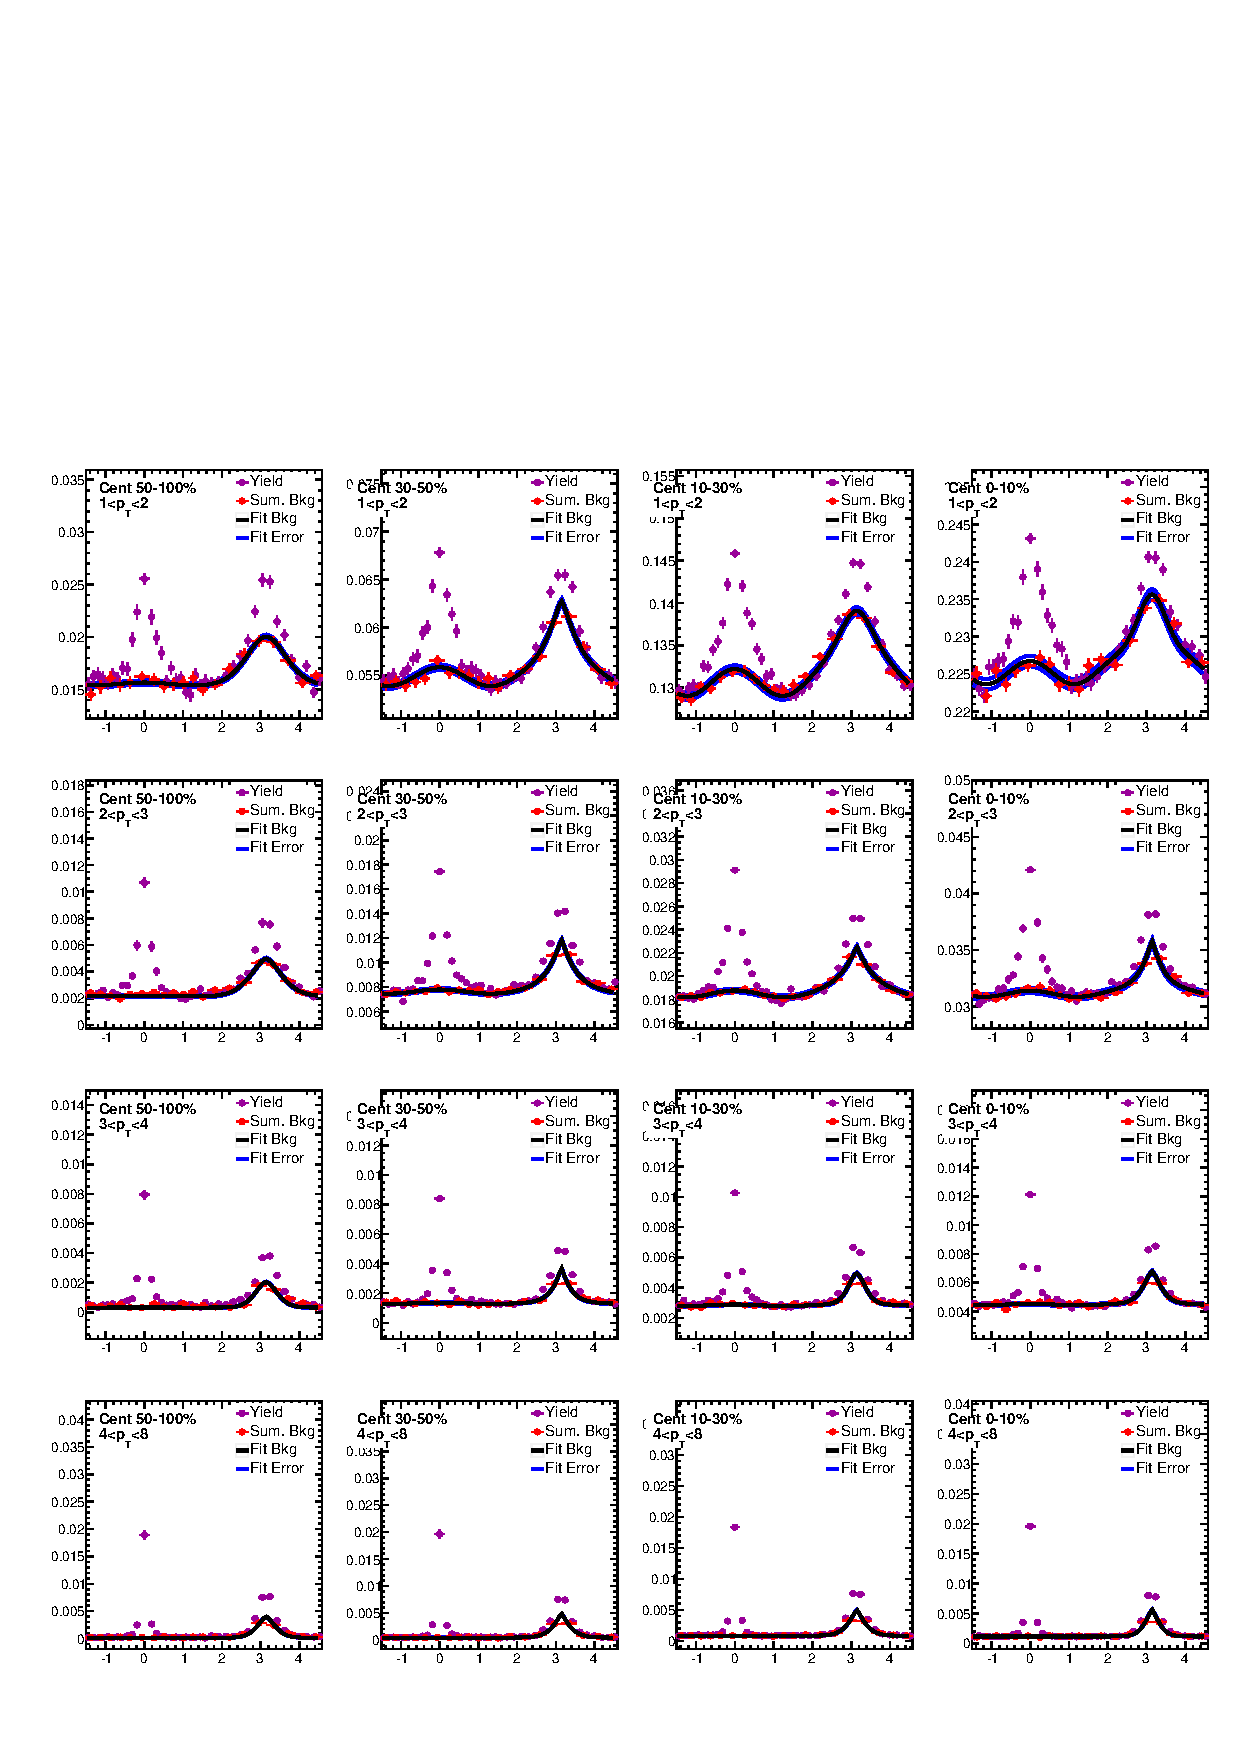
\includegraphics[width=0.9\textwidth]{figures/Appendices/Fits_PbPb_Leading.pdf}
\caption[Leading jet background fits]{Background leading jet $\Delta\phi$ distributions, estimated by projection over the region 1.5$<|\Delta\eta|<$3.0, is fit as shown.  The 2D background distripbution is estimated by propagating the black fit line in $\Delta\eta$, with uncertainty assigned by varying fit parameters by the appropriate fit error as shown in the blue error band.}
\end{center}
\end{figure}


\begin{figure}[hbtp]
\begin{center}
\includegraphics[width=0.9\textwidth]{figures/Appendices/Fits_PbPb_SubLeading.pdf}
\caption[Subleading jet background fits]{Background subleading jet $\Delta\phi$ distributions, estimated by projection over the region 1.5$<|\Delta\eta|<$3.0, is fit as shown.  The 2D background distribution is estimated by propagating the black fit line in $\Delta\eta$, with uncertainty assigned by varying fit parameters by the appropriate fit error as shown in the blue error band.}
\end{center}
\end{figure}

\begin{figure}[h!]
\begin{center}
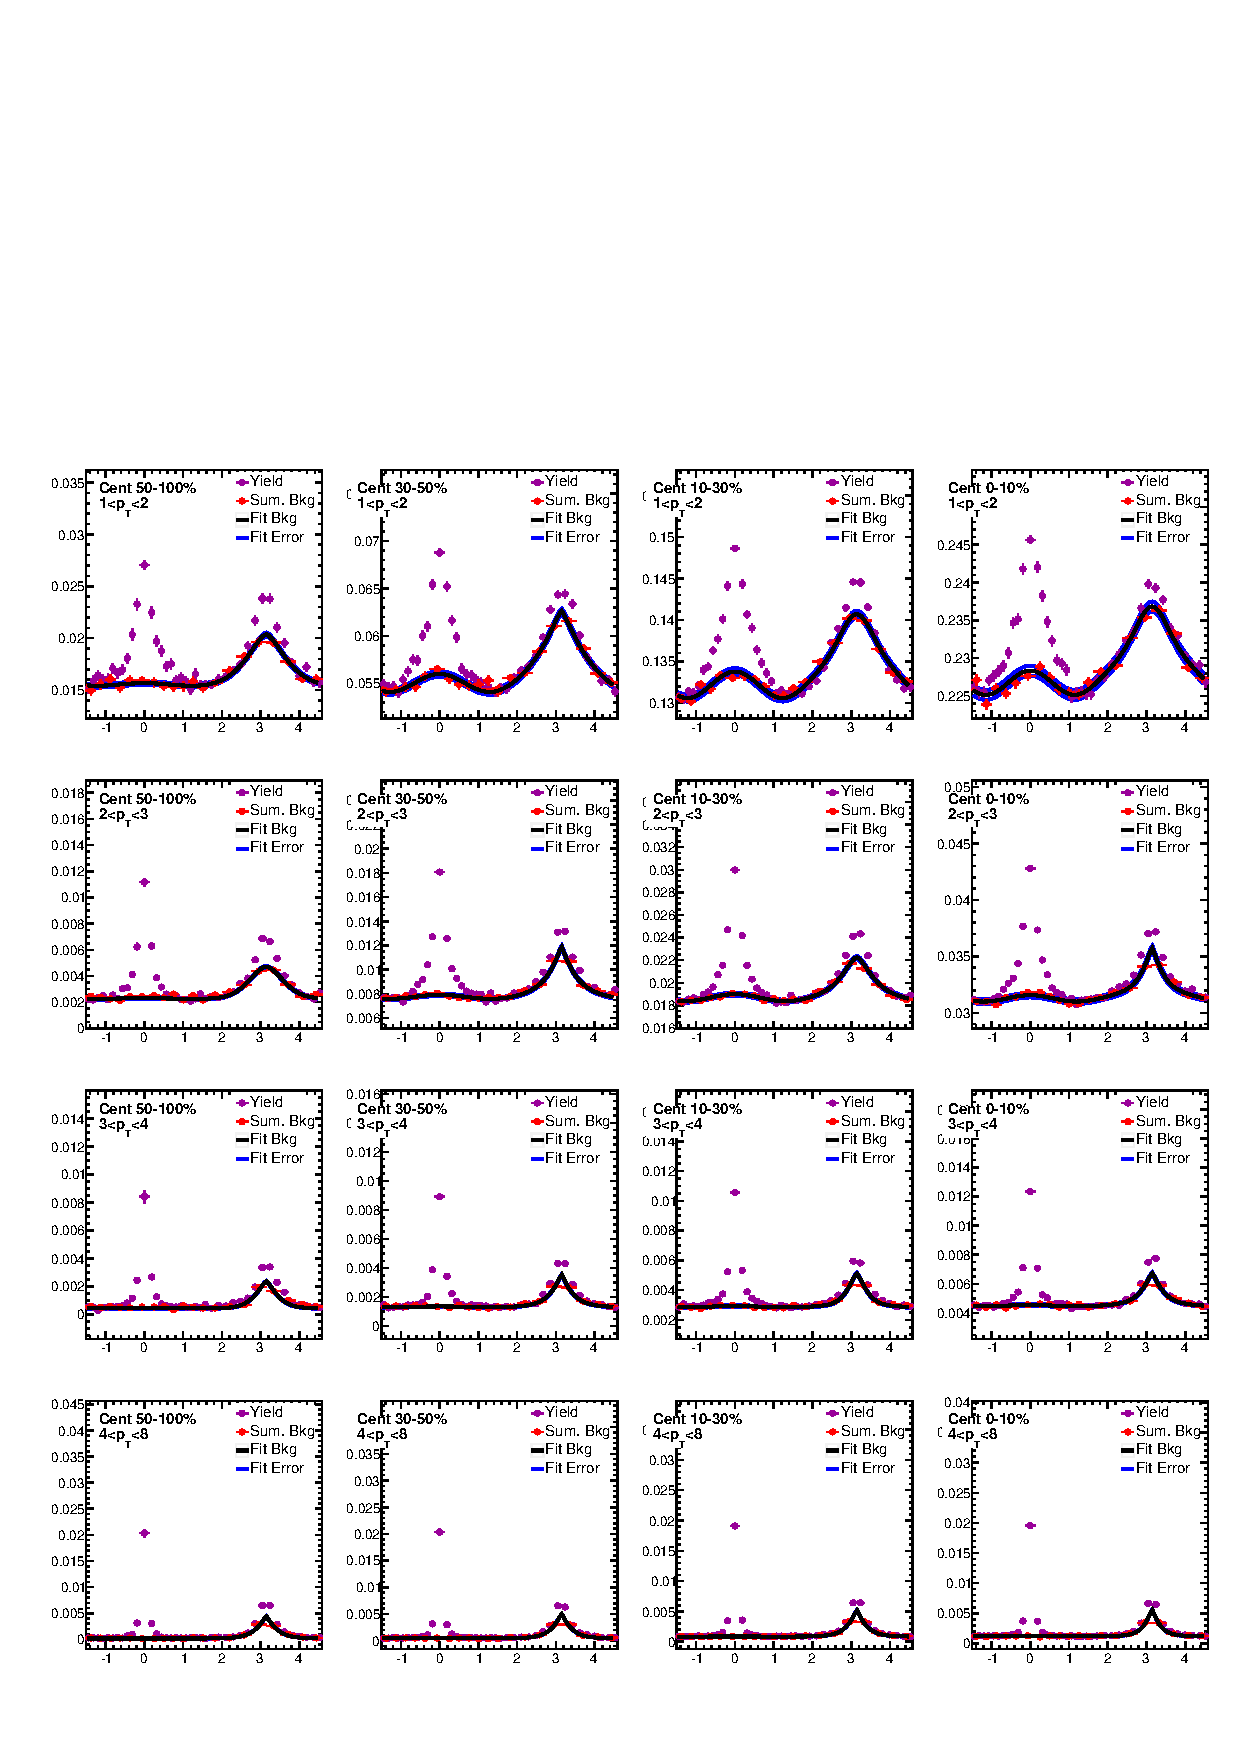
\includegraphics[width=0.9\textwidth]{figures/Appendices/Fits_PbPb_Inclusive.pdf}
\caption[Inclusive jet background fits]{Background inclusive jet $\Delta\phi$ distributions, estimated by projection over the region 1.5$<|\Delta\eta|<$3.0, is fit as shown.  The 2D background distribution is estimated by propagating the black fit line in $\Delta\eta$, with uncertainty assigned by varying fit parameters by the appropriate fit error as shown in the blue error band.}
\label{fig:inc_fit}
\end{center}
\end{figure}

\clearpage



\subsection{Pair acceptance and event decomposition systematic uncertainties}

\label{app:err_me_bkg}


Figure~\ref{fig:me_err} illustrates the estimation of pair-acceptance uncertainty, determined by considering the sideband asymmetry in the $\Delta\eta$ distributions of background subtracted yield.  

\begin{figure}[h!]
\begin{center}
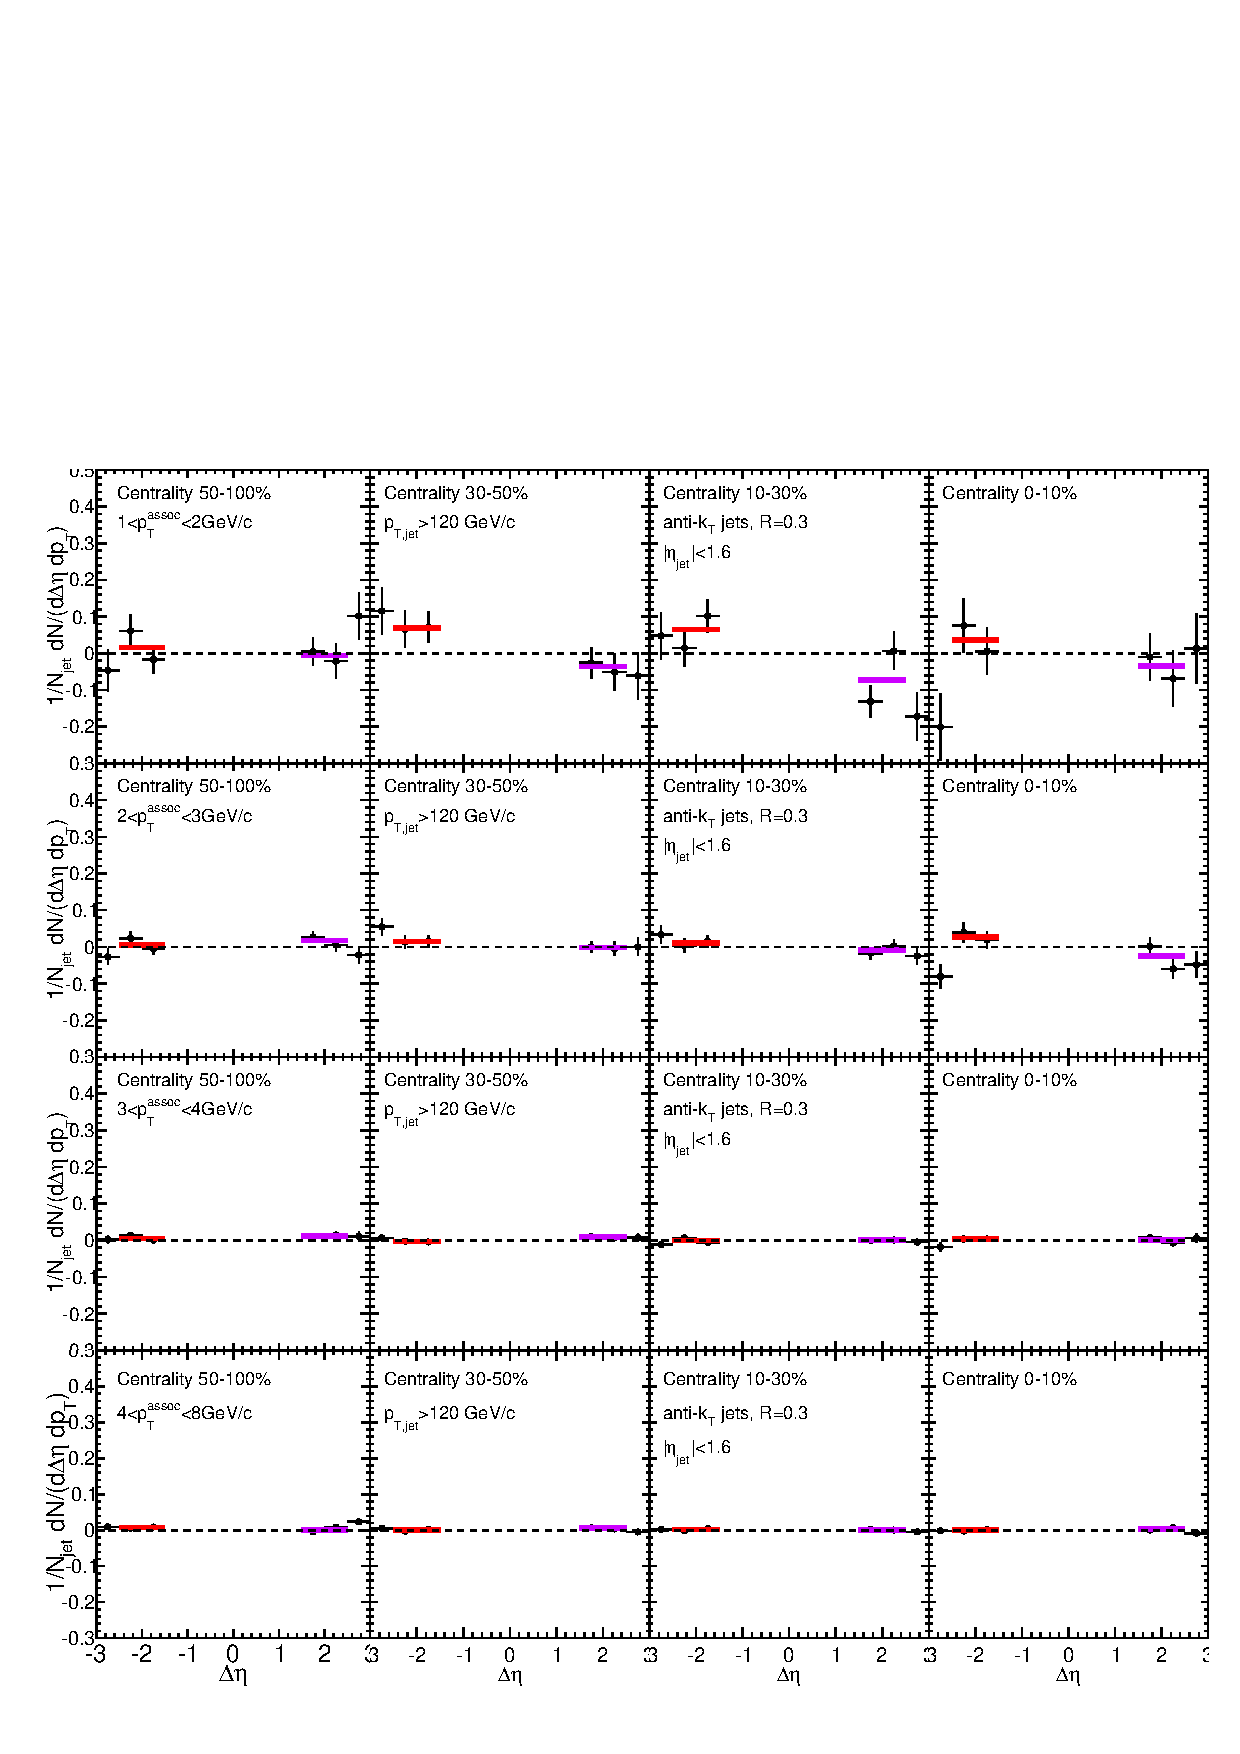
\includegraphics[width=0.9\textwidth]{figures/Appendices/Eta_EdgeFit_PbPb_Inclusive.pdf}
\caption[Pair acceptance uncertainty determination]{Background-subtracted inclusive jet $\Delta\eta$ distribution is shown for sideband region 1.5$<|\Delta\eta|<$3.0 only.  Each side is fit separately with a horizontal line, and the greater deviation from zero is assigned as systematic uncertainty arising from the pair-acceptance correction.}
\label{fig:me_err}
\end{center}
\end{figure}

\clearpage


\noindent Figure~\ref{fig:bkg_err} illustrates the background-subtraction systematic uncertainty estimation:  the average content of the two 1.5$<\Delta\eta<$2.0 bins is assigned as systematic uncertainty for each $p_{\rm T}$ and centrality bin.  

\begin{figure}[h!]
\begin{center}
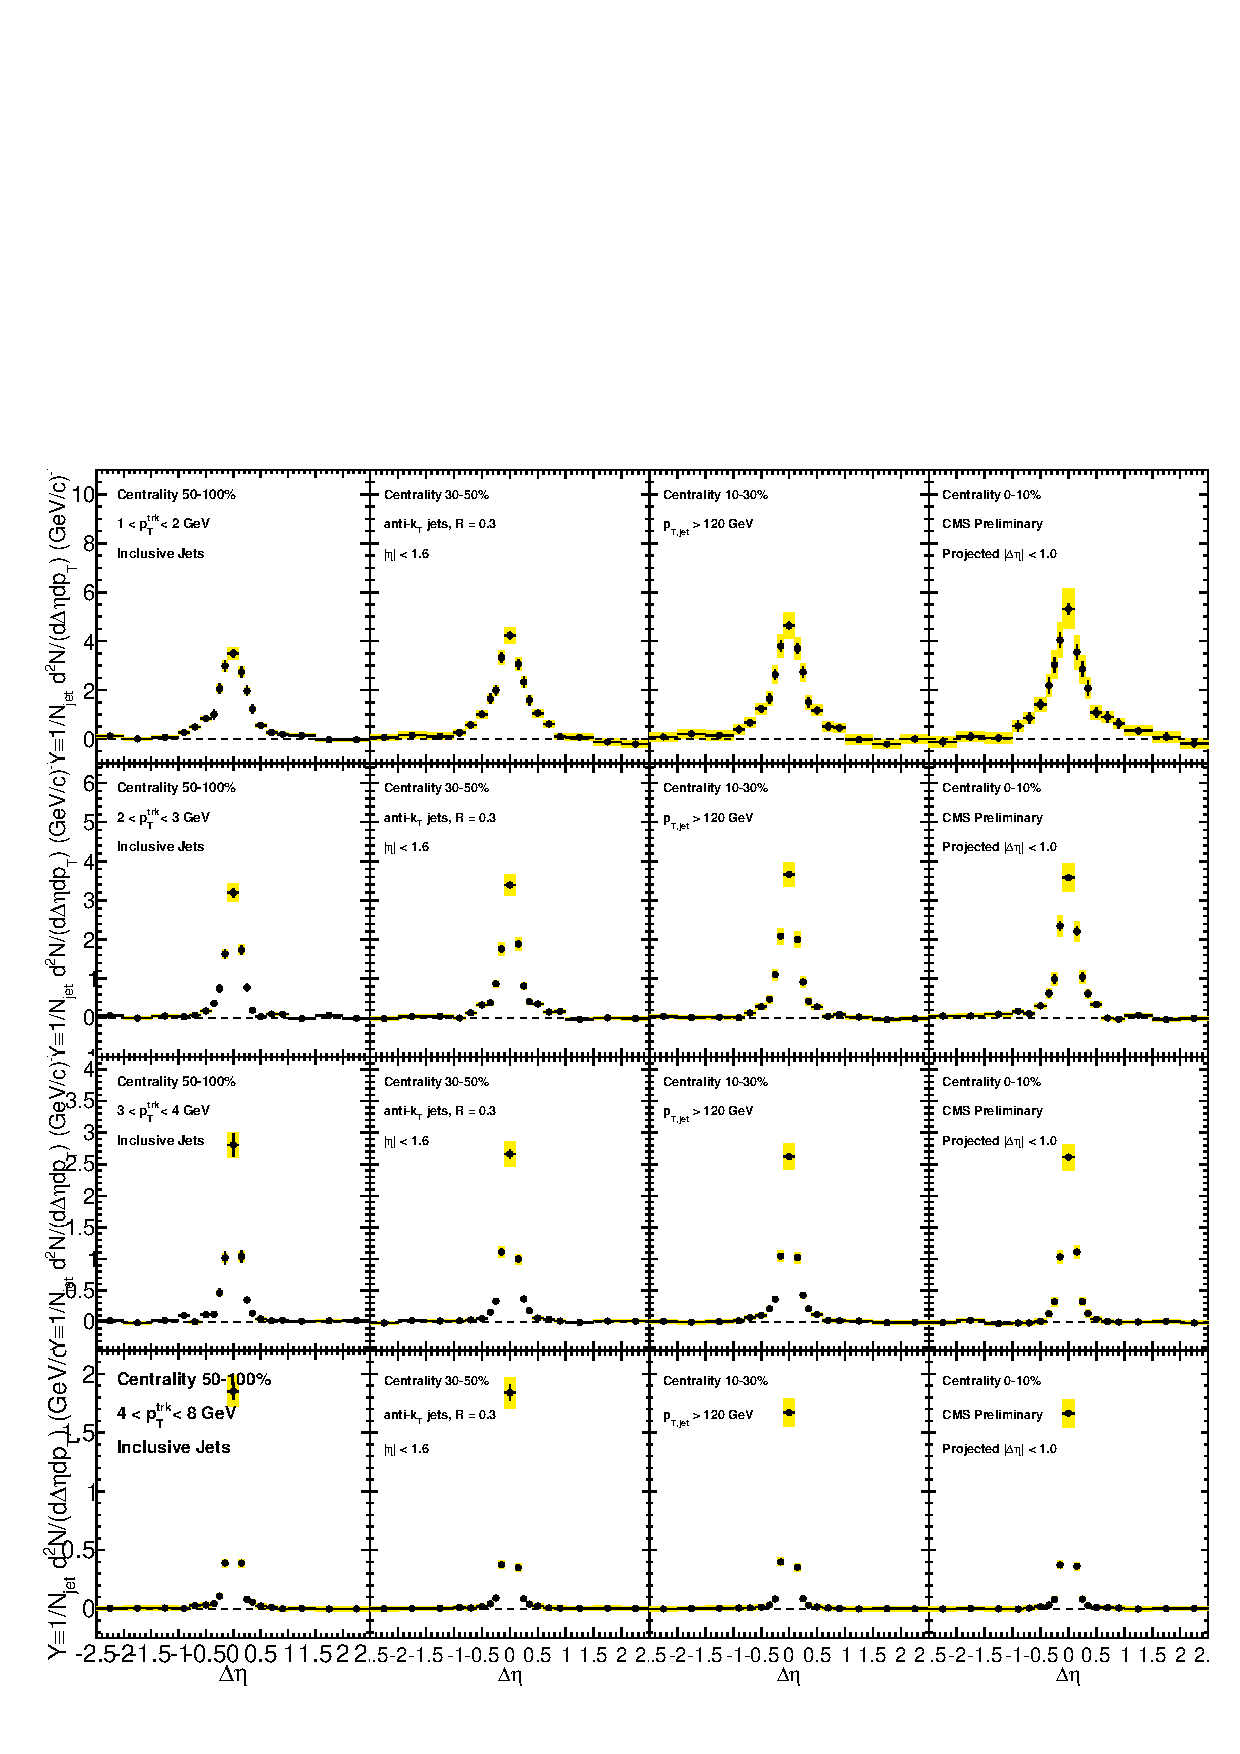
\includegraphics[width=0.9\textwidth]{figures/Appendices/Yield_Eta_wide_PbPb_Inclusive.pdf}
\caption[Background subtraction uncertainty determination]{Inclusive jet correlated yield in $\Delta\eta$, shown to axis range $|\Delta\eta|<2.0$.  The deviation of the most peripheral points from zero is assigned as systematic uncertainty as discussed in the Systematic Uncertainty section above.}
\label{fig:bkg_err}
\end{center}
\end{figure}
\clearpage



\subsection{Correlation widths and related uncertainty}

\label{app:width_determination}

\begin{figure}[h!]
\begin{center}

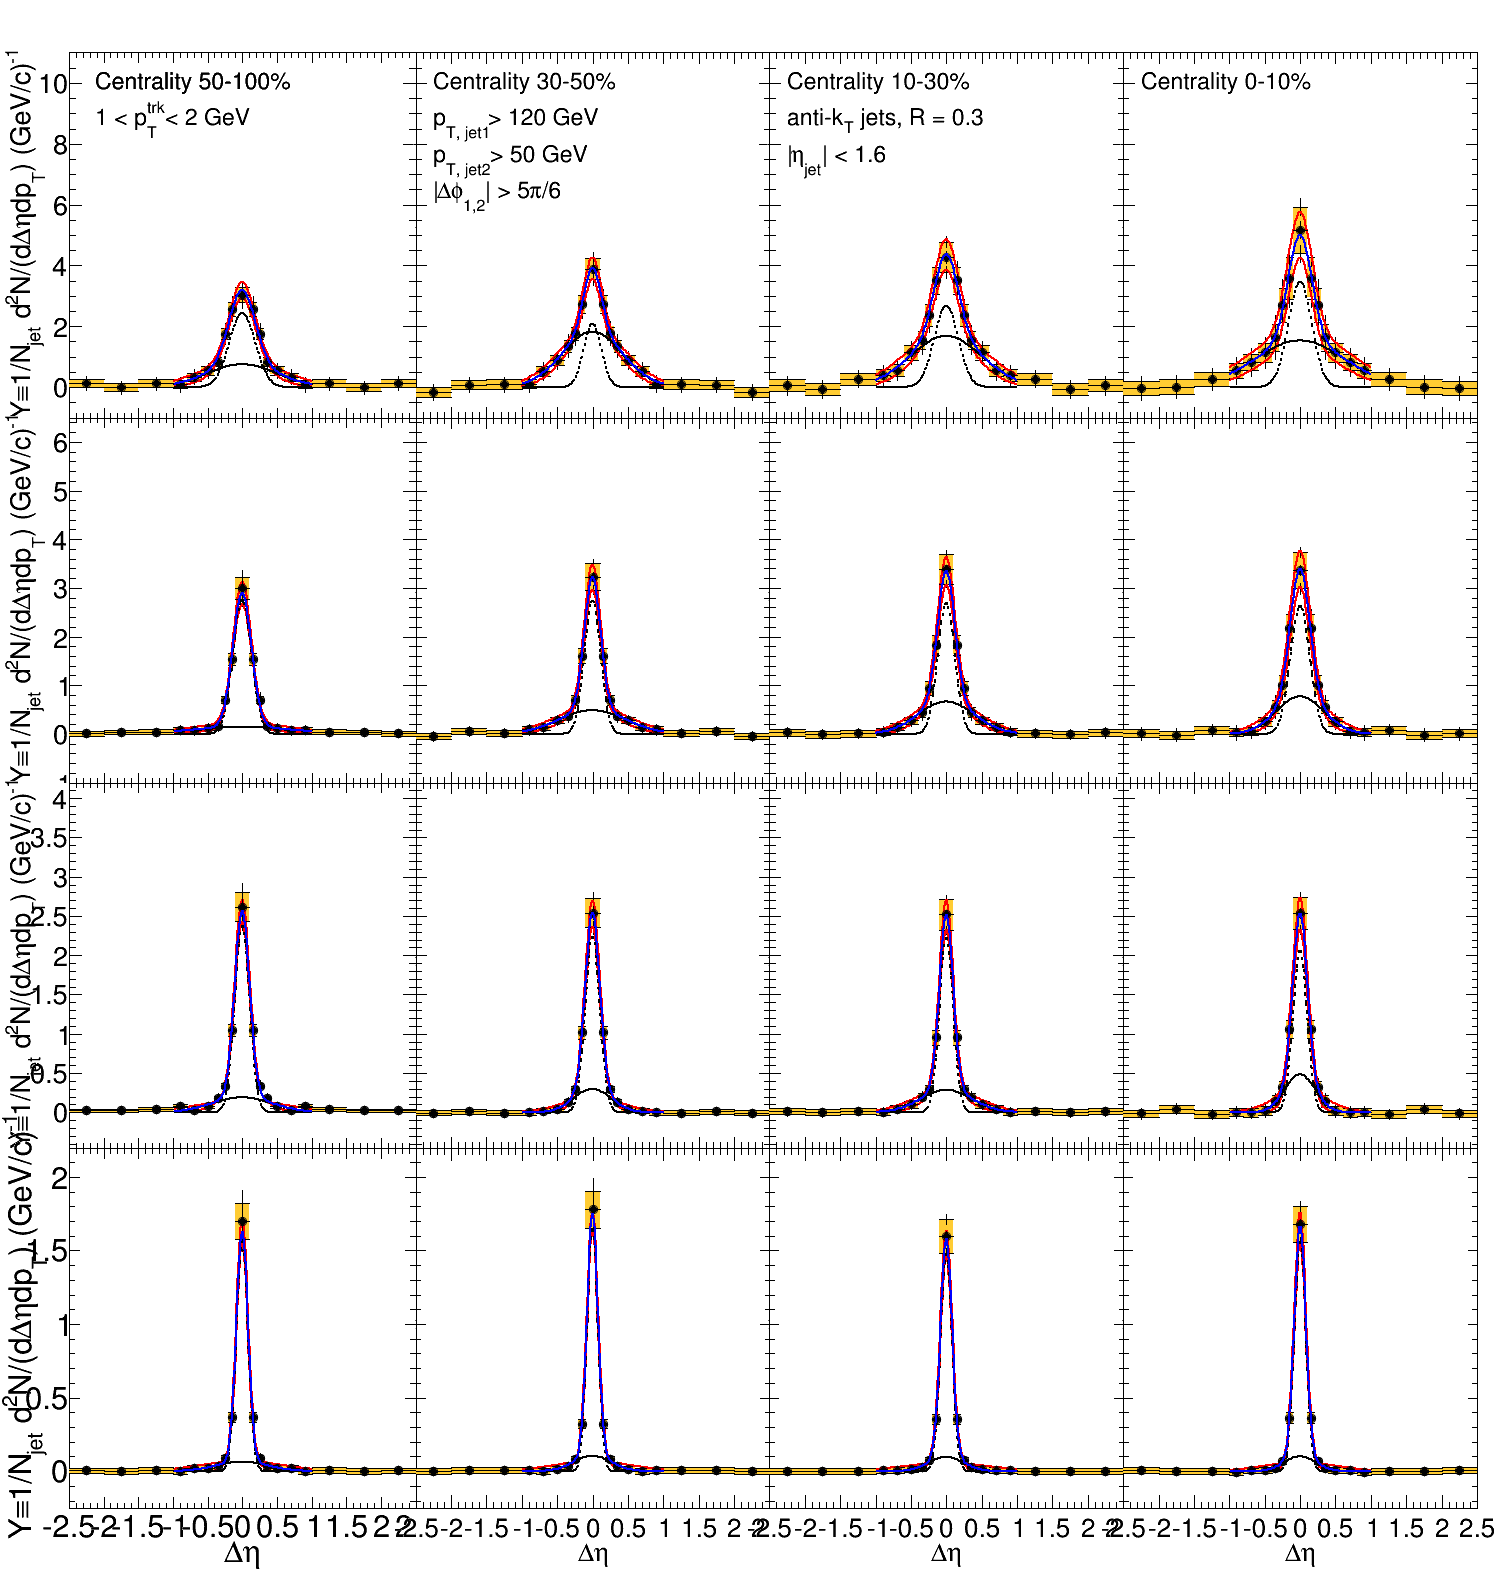
\includegraphics[width=0.9\textwidth]{figures/Appendices/Width_Check_Fits_Eta_PbPb_Leading.png}

\caption[Width determination for PbPb leading jets]{Illustration of the fits used to determine the distribution widths (shown here for leading jet PbPb $\Delta\eta$ correlations).  Correlations are fit to a double gaussian (shown in blue, with black dashed lines indicating constituent gaussians), and width is taken as the $\Delta\eta$ value containing 67\% of the total yield. Points are varied by their systematic errors and the fits are repeated (shown in red) to obtain the systematic error on the width.}
\label{fig:Width_check_fit_PbPb_lead}
\end{center}
\end{figure}



\begin{figure}[hbtp]
\begin{center}


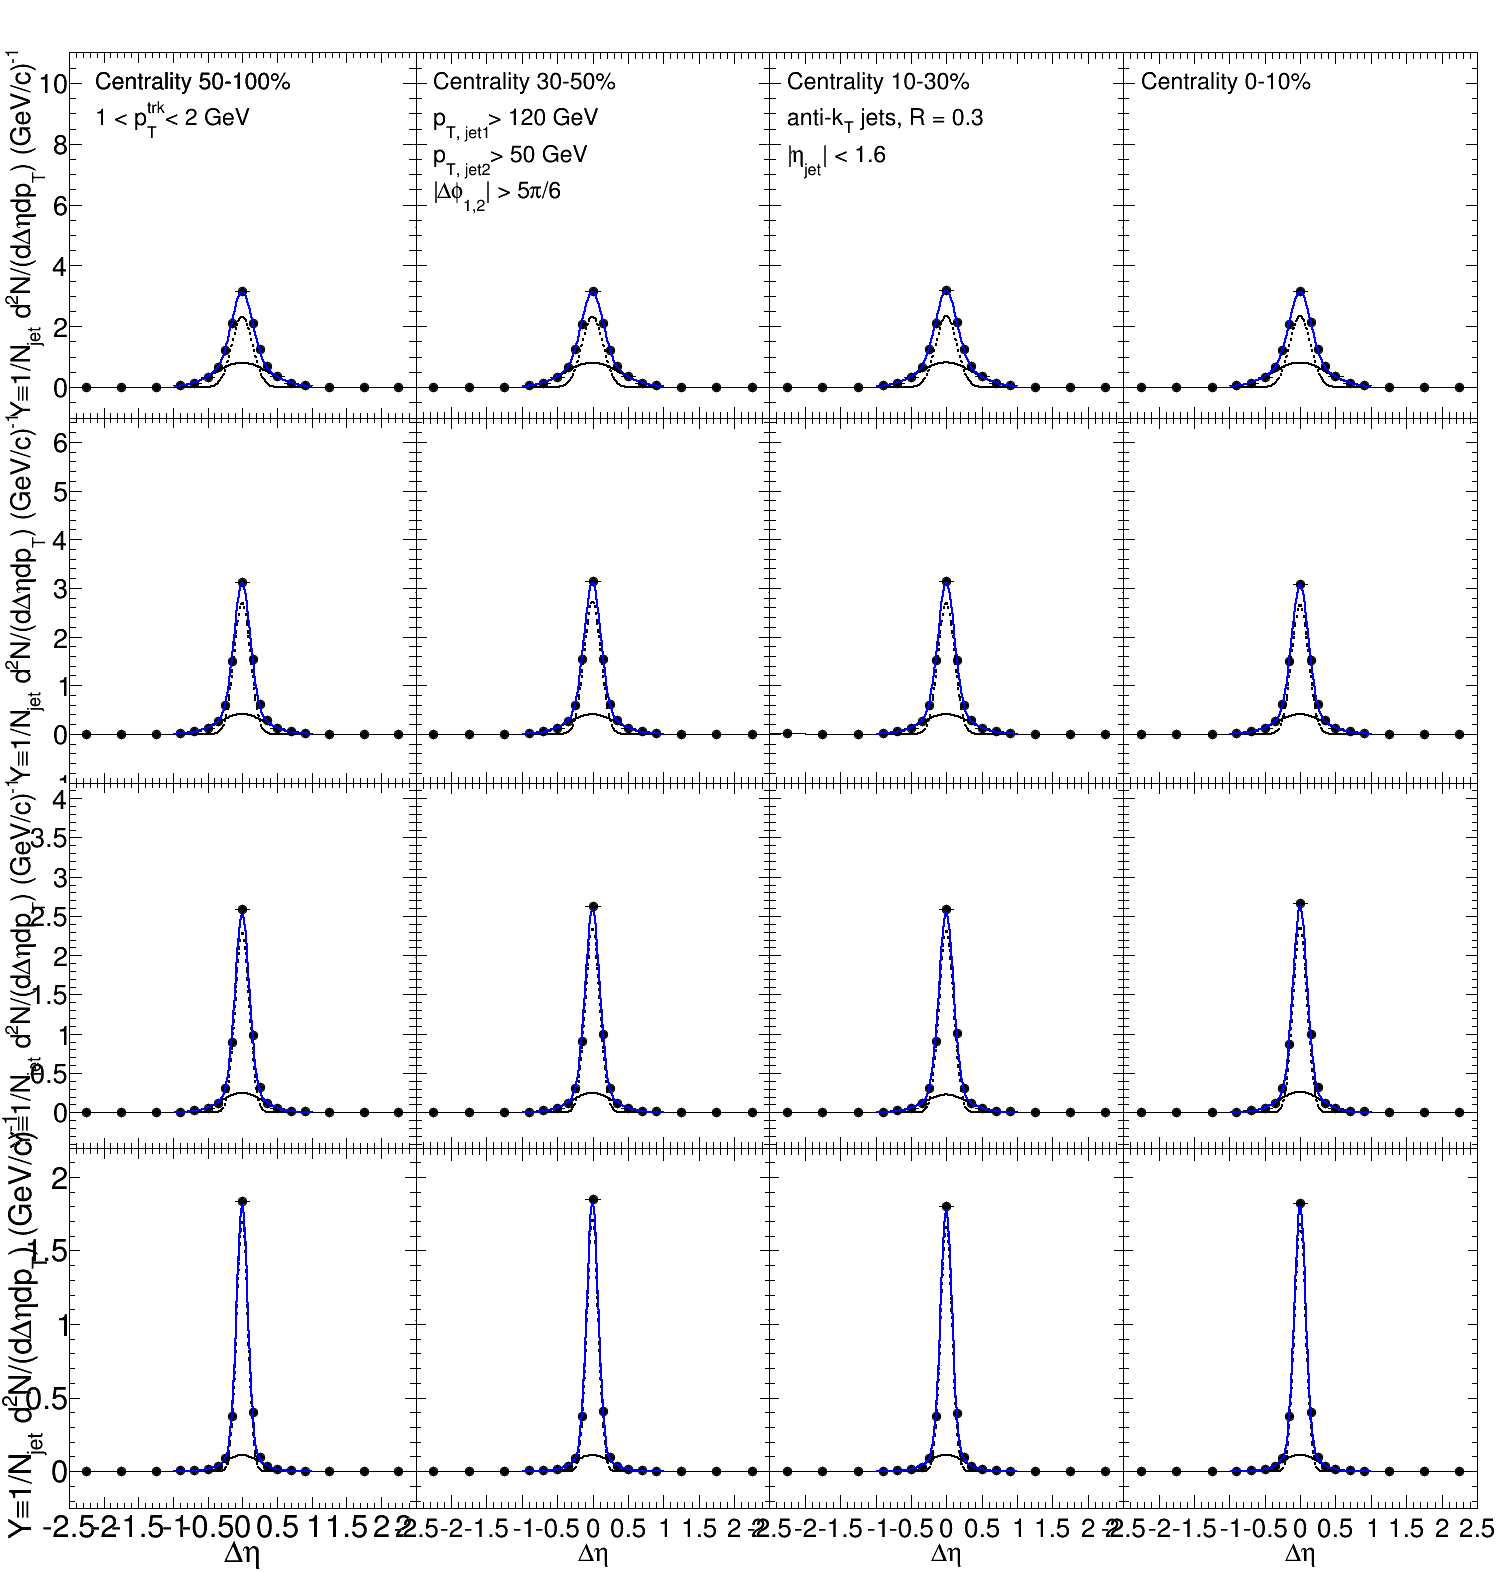
\includegraphics[width=0.9\textwidth]{figures/Appendices/Width_Check_Fits_Eta_pp_Leading.png}

\caption[Width determination for pp leading jets]{Illustration of the fits used to determine the distribution widths (shown here for leading jet pp $\Delta\eta$ correlations).  Correlations are fit to a double gaussian (shown in blue, with black dashed lines indicating constituent gaussians), and width is taken as the $\Delta\eta$ value containing 67\% of the total yield. }
\label{fig:Width_check_fit_pp_lead}
\end{center}
\end{figure}



\begin{figure}[hbtp]
\begin{center}

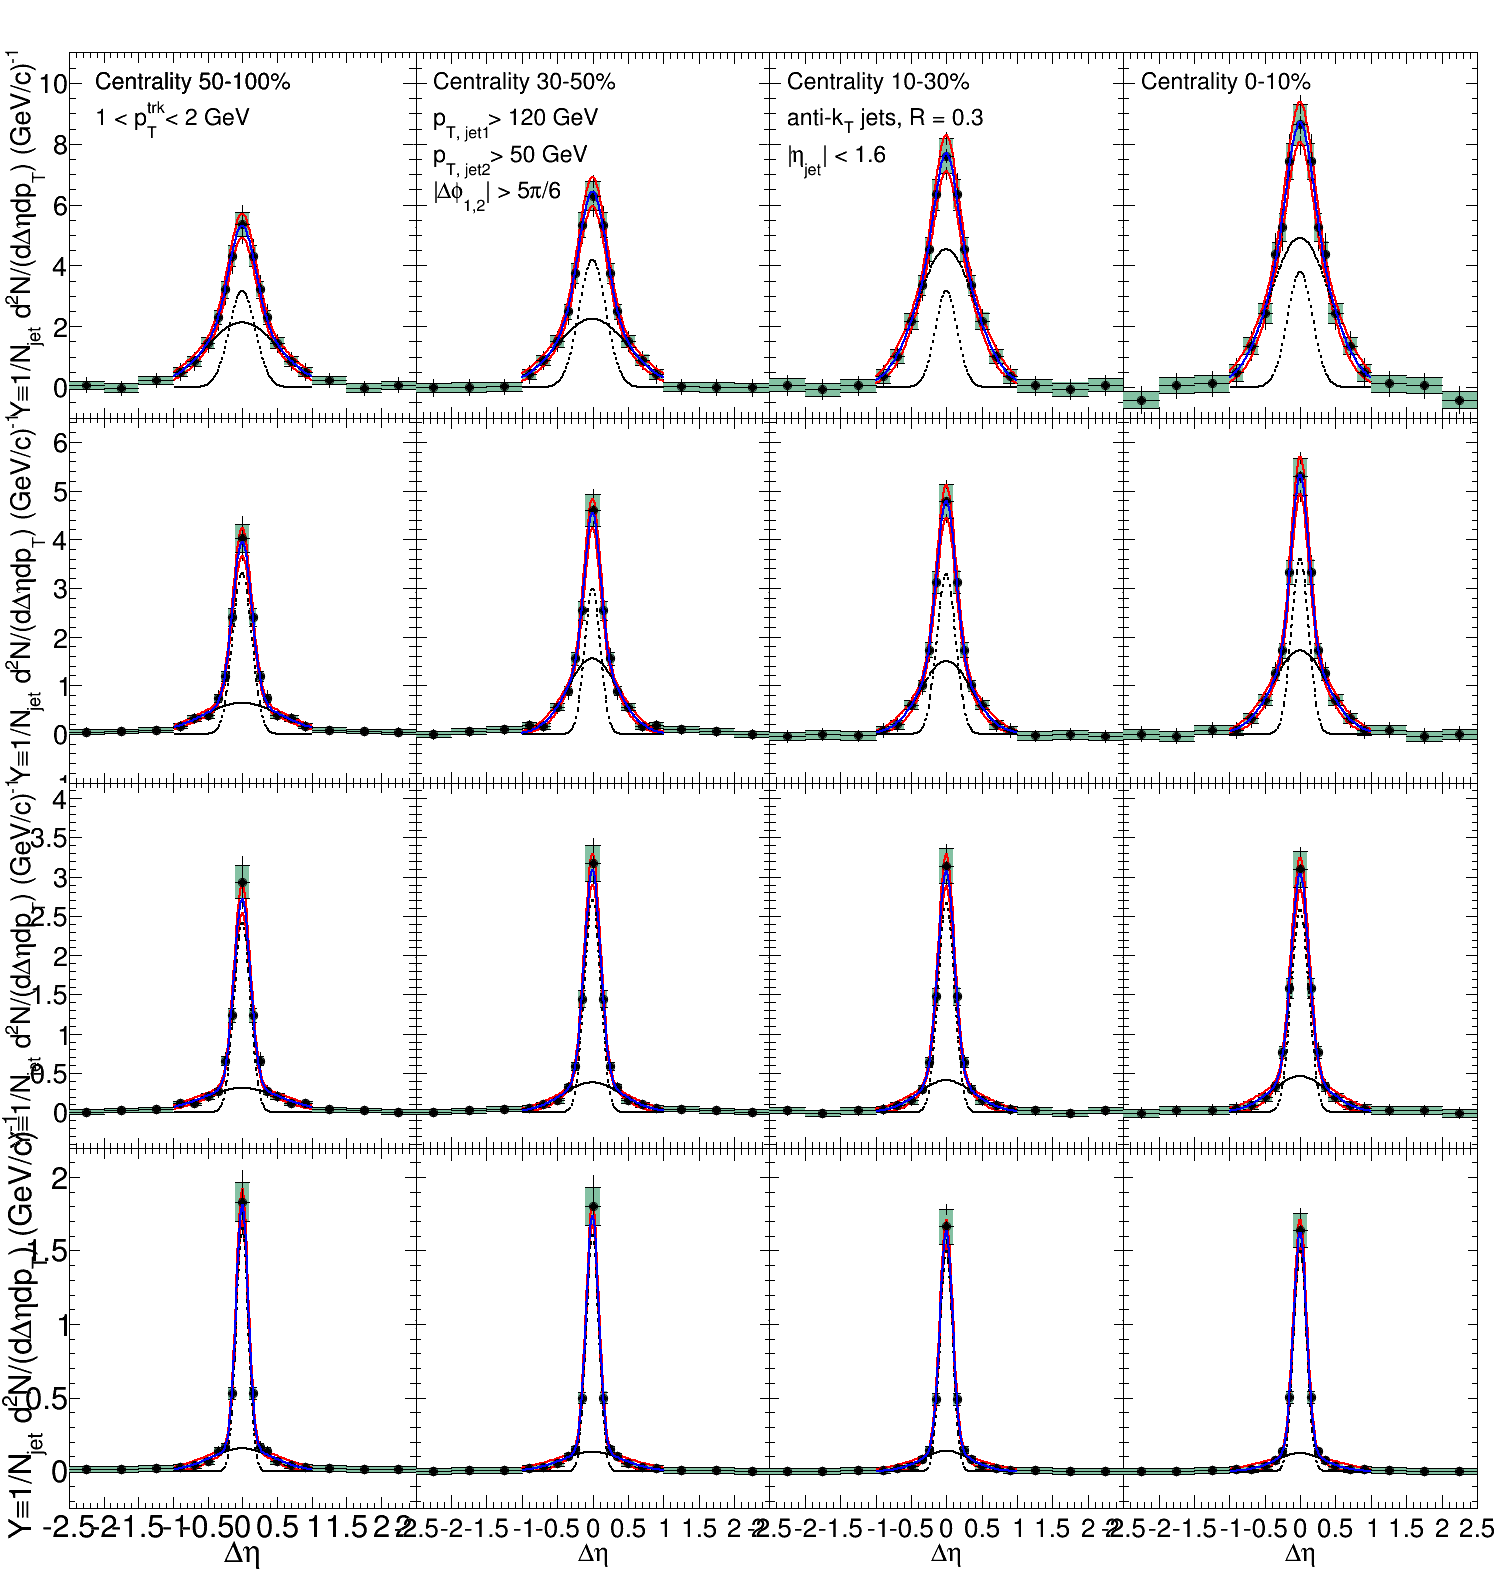
\includegraphics[width=0.9\textwidth]{figures/Appendices/Width_Check_Fits_Eta_PbPb_SubLeading.png}

\caption[Width determination for PbPb subleading jets]{Illustration of the fits used to determine the distribution widths (shown here for subleading jet PbPb $\Delta\eta$ correlations).  Correlations are fit to a double gaussian (shown in blue, with black dashed lines indicating constituent gaussians), and width is taken as the $\Delta\eta$ value containing 67\% of the total yield.  Points are varied by their systematic errors and the fits are repeated (shown in red) to obtain the systematic error on the width.}
\label{fig:Width_check_fit_PbPb_sublead}
\end{center}
\end{figure}


\begin{figure}[hbtp]
\begin{center}

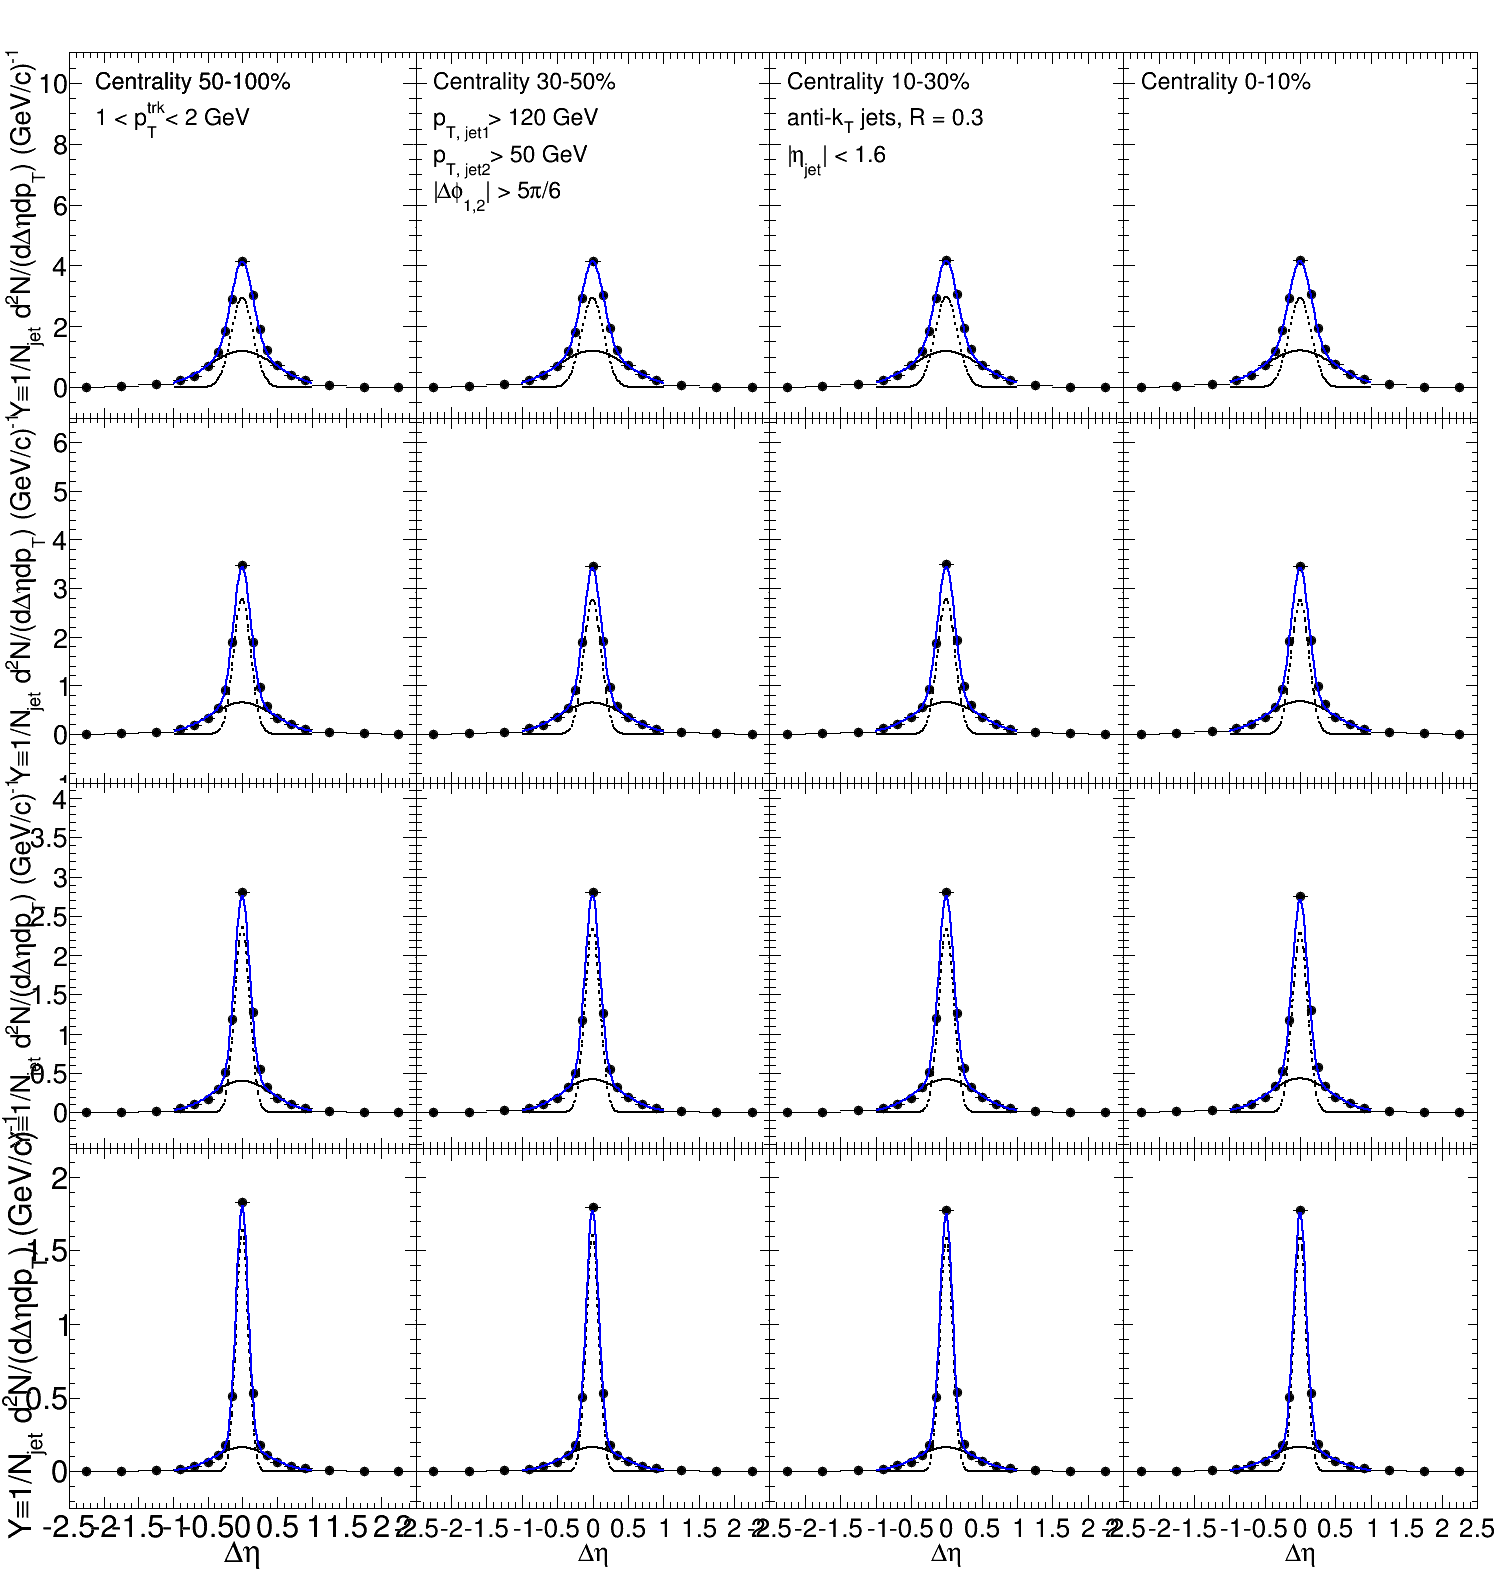
\includegraphics[width=0.9\textwidth]{figures/Appendices/Width_Check_Fits_Eta_pp_SubLeading.png}

\caption[Width determination for pp subleading jets]{Illustration of the fits used to determine the distribution widths (shown here for subleading jet pp $\Delta\eta$ correlations).  Correlations are fit to a double gaussian (shown in blue, with black dashed lines indicating constituent gaussians), and width is taken as the $\Delta\eta$ value containing 67\% of the total yield. }
\label{fig:Width_check_fit_pp_sublead}
\end{center}
\end{figure}

